
\documentclass[12pt,a4paper]{article}
\usepackage[latin1]{inputenc}
\usepackage{float}
\usepackage{amsmath}
\usepackage{amsfonts}
\usepackage{amssymb}
\usepackage{graphicx}
\usepackage[hidelinks]{hyperref}
\author{Luca Conterio - 920261\\
	Ibrahim El Shemy - 920174}
\date{A.Y. 2018/2019 - Prof. Di Nitto Elisabetta}



\title{%
	\textbf{\Huge{TrackMe}} \\
	\large Design Document
}

\begin{document}
	\begin{figure}
		\centering
		
\includegraphics[width=1.0\linewidth]{images/polimi}
	\end{figure}
	\maketitle

	\newpage
	\tableofcontents
	\newpage

	\section{Introduction}
	\subsection{Purpose}
	This document represents the \texttt{Design Document} (DD) for TrackMe software and contains a functional description of the system. We provide an overall guidance to the architecture of the system and it is therefore addressed to the software development team.
	\subsection{Scope}
	\texttt{TrackMe} is a company that wants to develop a software-based service allowing third parties to monitor the location and health status of individuals. Hence, the system has to be composed by two specific services:
	\begin{itemize}
	 	\item \textbf{Data4Help}\\\\
	 	This service supports the registration of individuals who agree that TrackMe acquires their data (through electronic devices such as smartwatches). Third Party will be able to access User's data (after their approval) and to request anonymized sampling searches.
	 	\item \textbf{AutomatedSOS}\\\\ 
	 	This service is oriented to elderly people: monitoring their health status parameters, the system can send to the location of the customer an ambulance when some parameters are below certain thresholds, guaranteeing a reaction time of less than 5 seconds from the time the parameters get lower than the threshold.
	\end{itemize}
 	\subsection{Definitions, Acronyms and Abbreviations}
 		\subsubsection{Definitions}
 			\begin{itemize}
 				\item \texttt{User Device}: any compatible device with the TrackMe application, either smartphone or smartwatch.
 				\item \texttt{Personal Information}: the collection of infromation provided by a User during the registration process. It Incudes legal information, such as Social Security Number, name, surname, birth date, address, e-mail address, mobile number. Sometimes in the document this expression is abbreviated by \texttt{Data}, that also refers to clinical data.
 				\item \texttt{Assistance Request}: it is a request formulated by the system and sent to the Ambulance Dispatching System in order to guarantee users the necessary assistance.
 				\item \texttt{Individual Access Request}: sometimes referred only as \texttt{individual request} or \texttt{access request}. It refers to a singular request sent by a Third Party to a User whenever it wants to have access to User's data. It needs the User's approval. 
 				\item \texttt{Sampling Search}: it refers to a search conducted by a Third Party according to some filters, returning anonymized results for a group of people. In this document it is often called only \texttt{sampling}.
 				\item \texttt{Mobile App}: an application that can be run by mobile devices, both smartphones and smartwatches.
 				\item \texttt{External Service}: a service provided by some components/modules through an API that is not needed to be implemented, since it is already available.
 			\end{itemize}
 		\subsubsection{Acronyms}
 			\begin{itemize}
 				\item \textbf{DD}: Design Document
 				\item \textbf{RASD}: Requirments Analysis and Specification
 				\item \textbf{ERP}: Enterprise Resource Planning
 				\item \textbf{DMZ}: Demilitarized Zone
 				\item \textbf{RAPS}: Reliable Array of Partitioned Service
 				\item \textbf{API}: Application Programming Interface
 				\item \textbf{DBMS}: Database Management System
 				\item \textbf{SMS}: Short Message Service
 			\end{itemize}
 		\subsubsection{Abbreviations}
 			\begin{itemize}
 				\item {[}Gn{]}: n-goal.
 				\item {[Rn]}: n-requirment.
 				\item {[Rx] - [Ry]}: from x-th requirement to y-th requirement.
 				\item {App}: application.
 			\end{itemize}
 		
 	\newpage
	\subsection{Document Structure}
		\begin{itemize}
			\item \textbf{1 Introduction}\\\\
			This section introduces the Design Document. It explains the Purpose, the Scope and the framework of the document.
			\item \textbf{2 Architectural Design}\\\\
			This section is focused on the main components used for this system and the relationship between them, providing information about their deployment and how they operate. It also focuses on the architectural styles and the design patterns adopted for designing the system.
			\item \textbf{3 User Interface Design}\\\\
			This section provides an overview on how the User Interface will look like. In our case this section won't be detailed since all the product functions have been already represented in the RASD.
			\item \textbf{4 Requirments Traceability}\\\\
			This section explains how the requirements defined in the RASD map to the design elements defined in this document.
			\item \textbf{5 Implementation, Integration and Test Plan}\\\\
			In this section we identify the order in which we plan to implement the subcomponents of the system and the order in which we plan to integrate and test them.
		\end{itemize}
\newpage
\section{Architectural Design}
	\subsection{High Level Components and their Interactions}
	\begin{figure}[h]
		\centering
		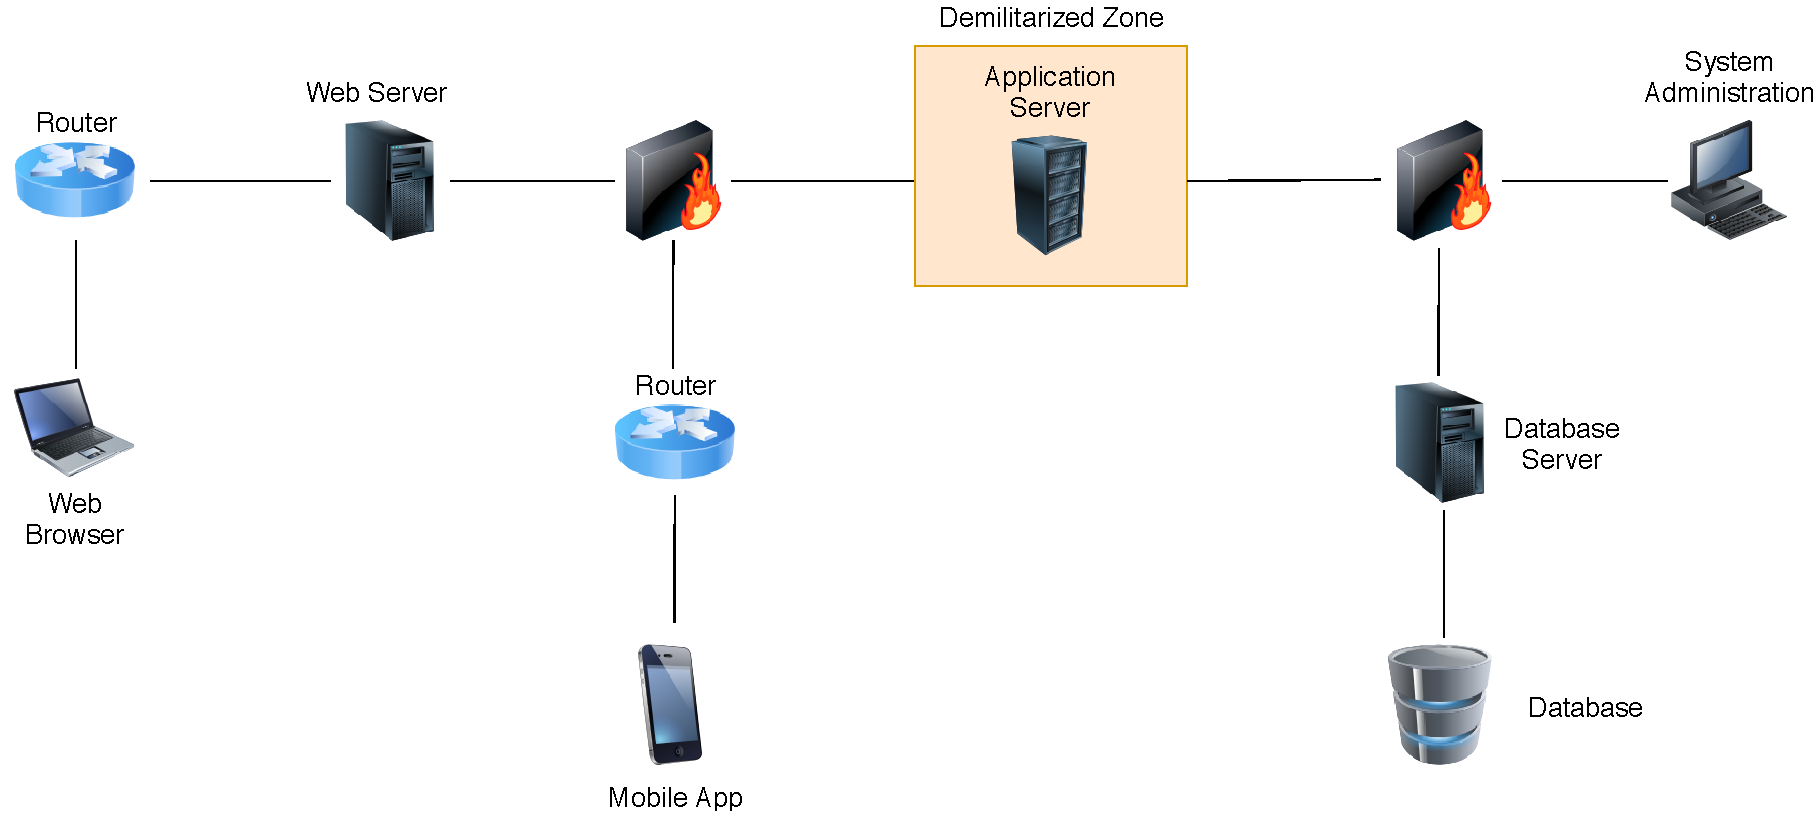
\includegraphics[height=0.5\linewidth]{images/high_level_diag}
		\caption{High Level System Structure}
		\label{fig:highleveldiag} 
	\end{figure}


The architecture of our system can be streamlined into 3 logic layers:
	\begin{itemize}
		\item \textbf{Presentation Layer}\\ 
		This layer can be divided into the Client tier (that includes the Web App and the Mobile App) and the Web tier. Third parties can access the system's functionalities and Users' information to which they are subscribed to through the Web Server. 
		\item \textbf{Application Layer}\\
		Users logged into the Mobile Application can access the system's functionalities and communicate with the Application Server, located in a Demilitarized Zone (DMZ), directly.
		\item \textbf{Data Layer}\\
		On top of that, we have the Database Server and the Database itself, where data about registered Users and Third Parties are stored and managed.
	\end{itemize}
	System Administration is implemented through a third-party ERP solution, hence we do not provide information about its implementation.
	
	\subsection{Component View}
		\subsubsection{High Level Component Diagram}	
			The following diagrams illustrate the system components and the interfaces through which they interact to fullfil their functionalities. A distinction can be made between Client side and Server side:
			\begin{itemize}
				\item The Client side is composed by two components, \texttt{Web Application} and \texttt{Mobile Application},  referring to the following services:\\
				\texttt{ThirdPartiesWebServices} and \texttt{UserMobileServices}.
				
				\item The Server side is composed of two main components, \texttt{Third Parties web services} that will provide functionalities aiming to fullfill third parties needs, such as sending requests to Users, \texttt{User mobile services} that will provide an interface to User in order to manage his own profile, check information about his health status, accept/reject requests, etc.
			\end{itemize}
			
			\begin{figure}[h]
				\centering
				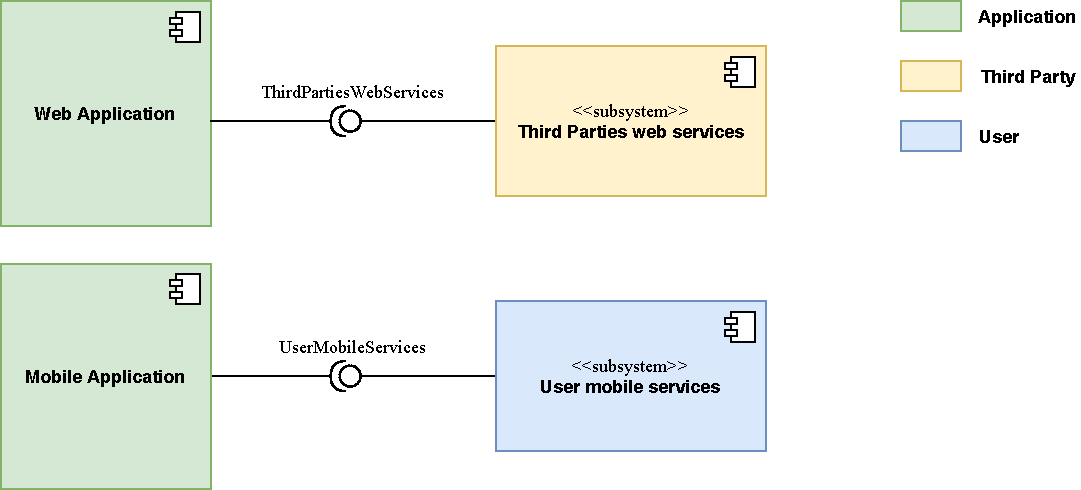
\includegraphics[width=1.0\linewidth]{images/high_lvl_comp_diag}
				\label{fig:highlvlcompdiag}
			\end{figure}
	
		\newpage
		\subsubsection{User Mobile Services Projection}
			User Mobile Services subsystem is composed by five components: \texttt{Activity Tracker Module}, \texttt{Health Monitoring Module}, \texttt{SOS Assistance Module}, \texttt{Access Requests Module} and \texttt{Profile Manager Module}. These components provide to the User Mobile Application the following interfaces: \texttt{ActivityTracker}, \texttt{HealthMonitor}, \texttt{AssistanceRequestHandler}, \texttt{RequestHandler} and \texttt{ProfileManager}. The components need also to communicate with a \texttt{Maps Service}, a \texttt{Sensors Service}, a \texttt{Notifications Service}, the \texttt{Ambulance Dispatching System}, a \texttt{SMS Service} and the \texttt{DBMS} to work properly and guarantee a better User experience with the Application.
			\begin{figure}[H]
				\centering
				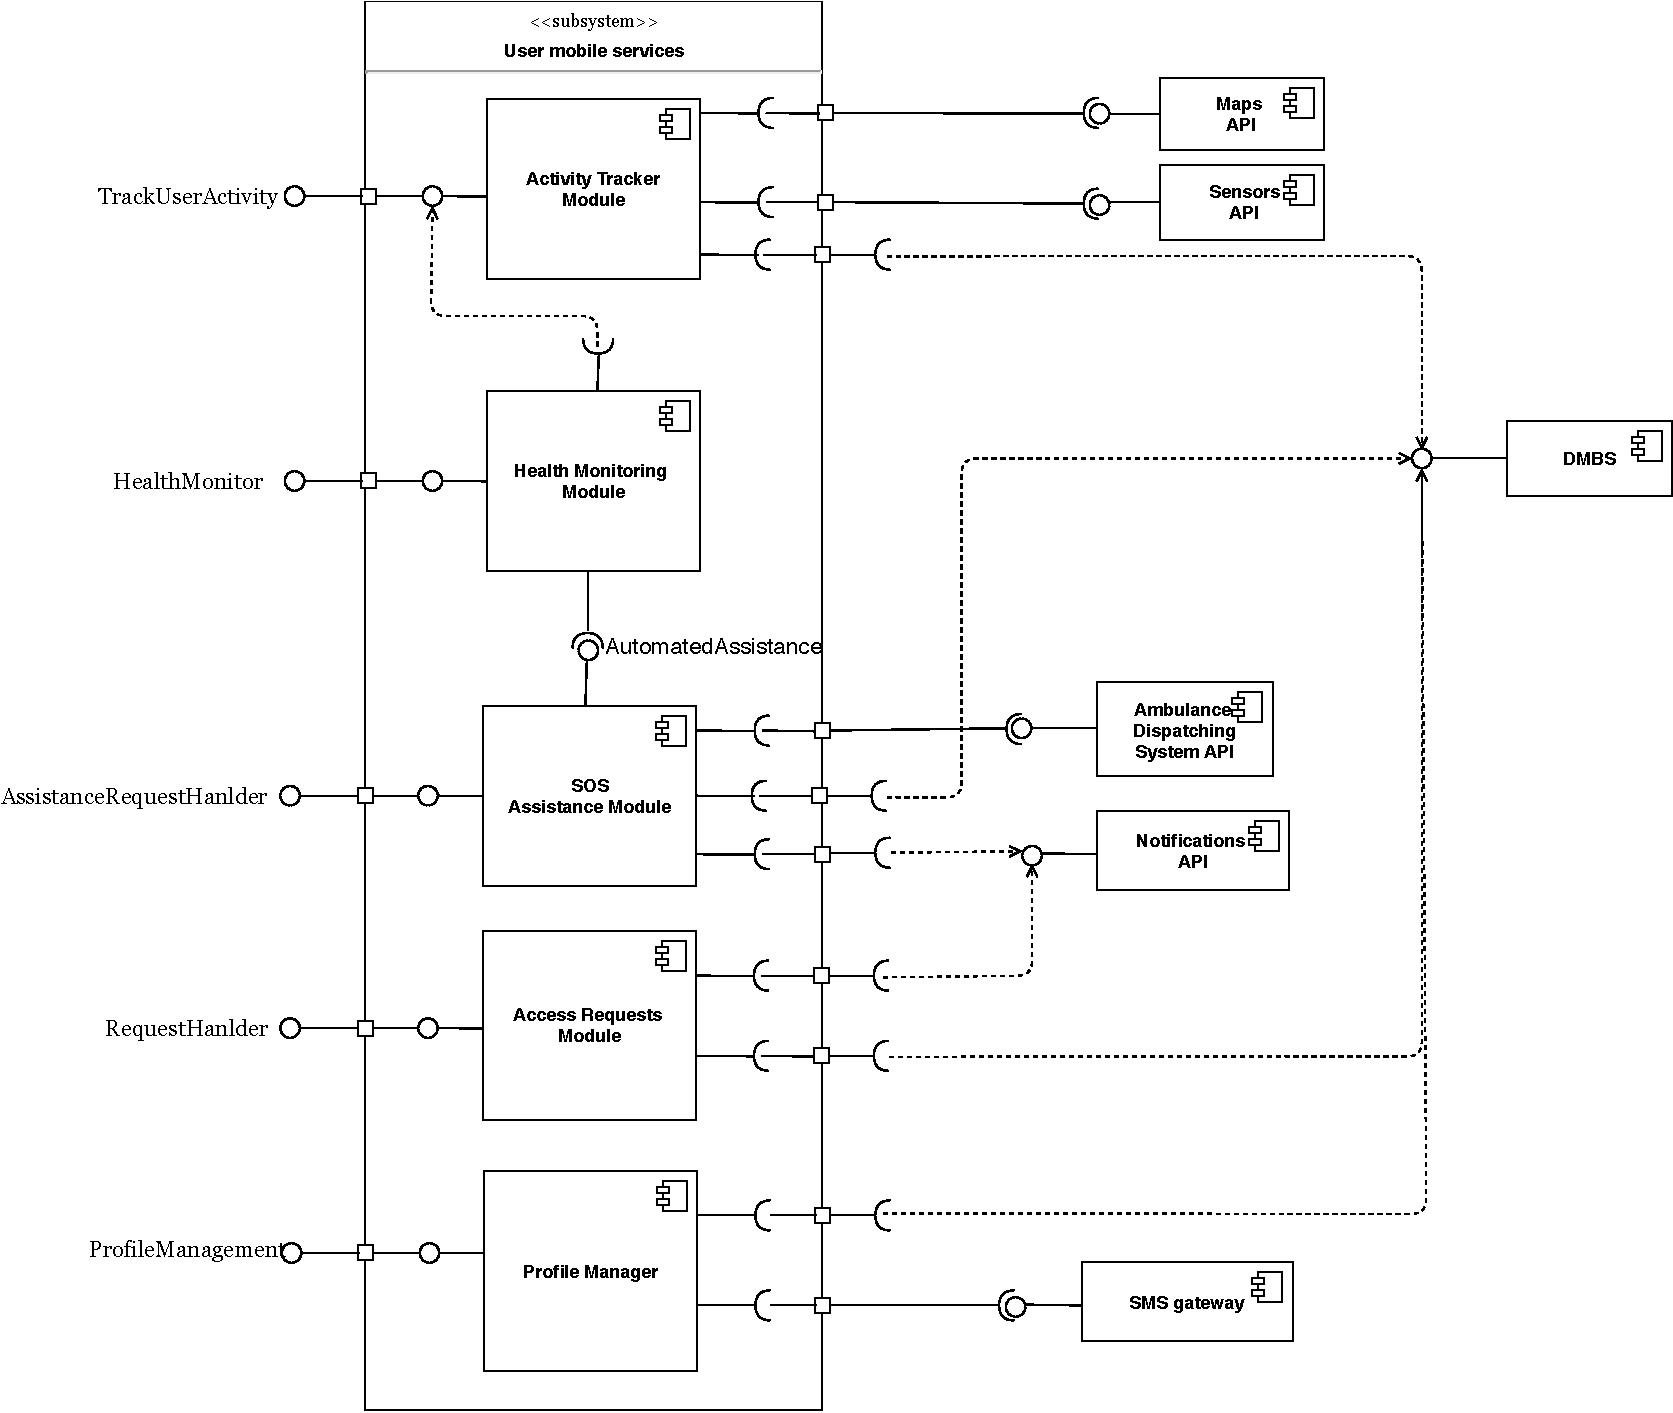
\includegraphics[height=1.0\linewidth]{images/user_projection}
				\label{fig:user_projection}
			\end{figure}
			\newpage
			For what concerns smartwatches, the server will not distinguish between messages and requests received directly by the smartwatch device (e.g. if it is equipped with GPS) and those retrieved by the sensors and forwarded to the server thanks to the connectivity of a smartphone.
			The User Mobile Services subsystem will handle all the mentioned situations.\\
			The only difference is that the smartwatch interface will not provide the user the possibility to manage his/her profile, since it would not be user friendly nor comfortable.
		
			\subsubsection*{Module Functionalities}
				\begin{itemize}
					\item \texttt{Activity Tracker Module}: this module is devoted to everything that concerns data retrieved by user's devices, such as location, steps, covered distance, heartbeat, blood pressure and sleep.
					\item \texttt{Health Monitoring Module}: this component persists in an idle state as long as a user is not registered to AutomatedSOS service.\\
					Otherwise, it interpellates directly the Activity Tracker Module, through the ActivityTracker interface in order to check the user's health status. Moreover, thanks to the AutomatedAssistance interface it can ask for an automated assistance request.
					\item \texttt{SOS Assistance Module}: in this module all functions dealing with assistance requests are implemented. It directy handles on-demand assistance requests and automated assistance requests performed by the Health Monitoring Module through the AutomatedAssistance interface.
					\item \texttt{Access Requests Module}: this component handles the access requests coming from some third parties, that want to have access to the user's data, giving the user the possibility to accept or reject them. It also manages the updates performed by the user to the permissions given to the third parties.
					\item \texttt{Profile Manager Module}: it provides all the functions concerning the user authentication and the update of profile informations.
				\end{itemize}
		
		\newpage
		\subsubsection{Third Party Web Services Projection}
				 Third Party Web Services subsystem is composed by five components: \texttt{Data Access Module}, \texttt{Subscription Module}, \texttt{Individual Requests Module}, \texttt{Sampling Requests Module} and \texttt{Authentication Manager Module}. These components provide to the Web Application the following interfaces: \texttt{DataAccessManager}, \texttt{SubscriptionManager}, \texttt{RequestProvider} and \texttt{AuthenticationManager}. The components need also to communicate with a \texttt{Notifications Service} and the \texttt{DBMS} to work properly.
			\begin{figure}[H]
				\centering
				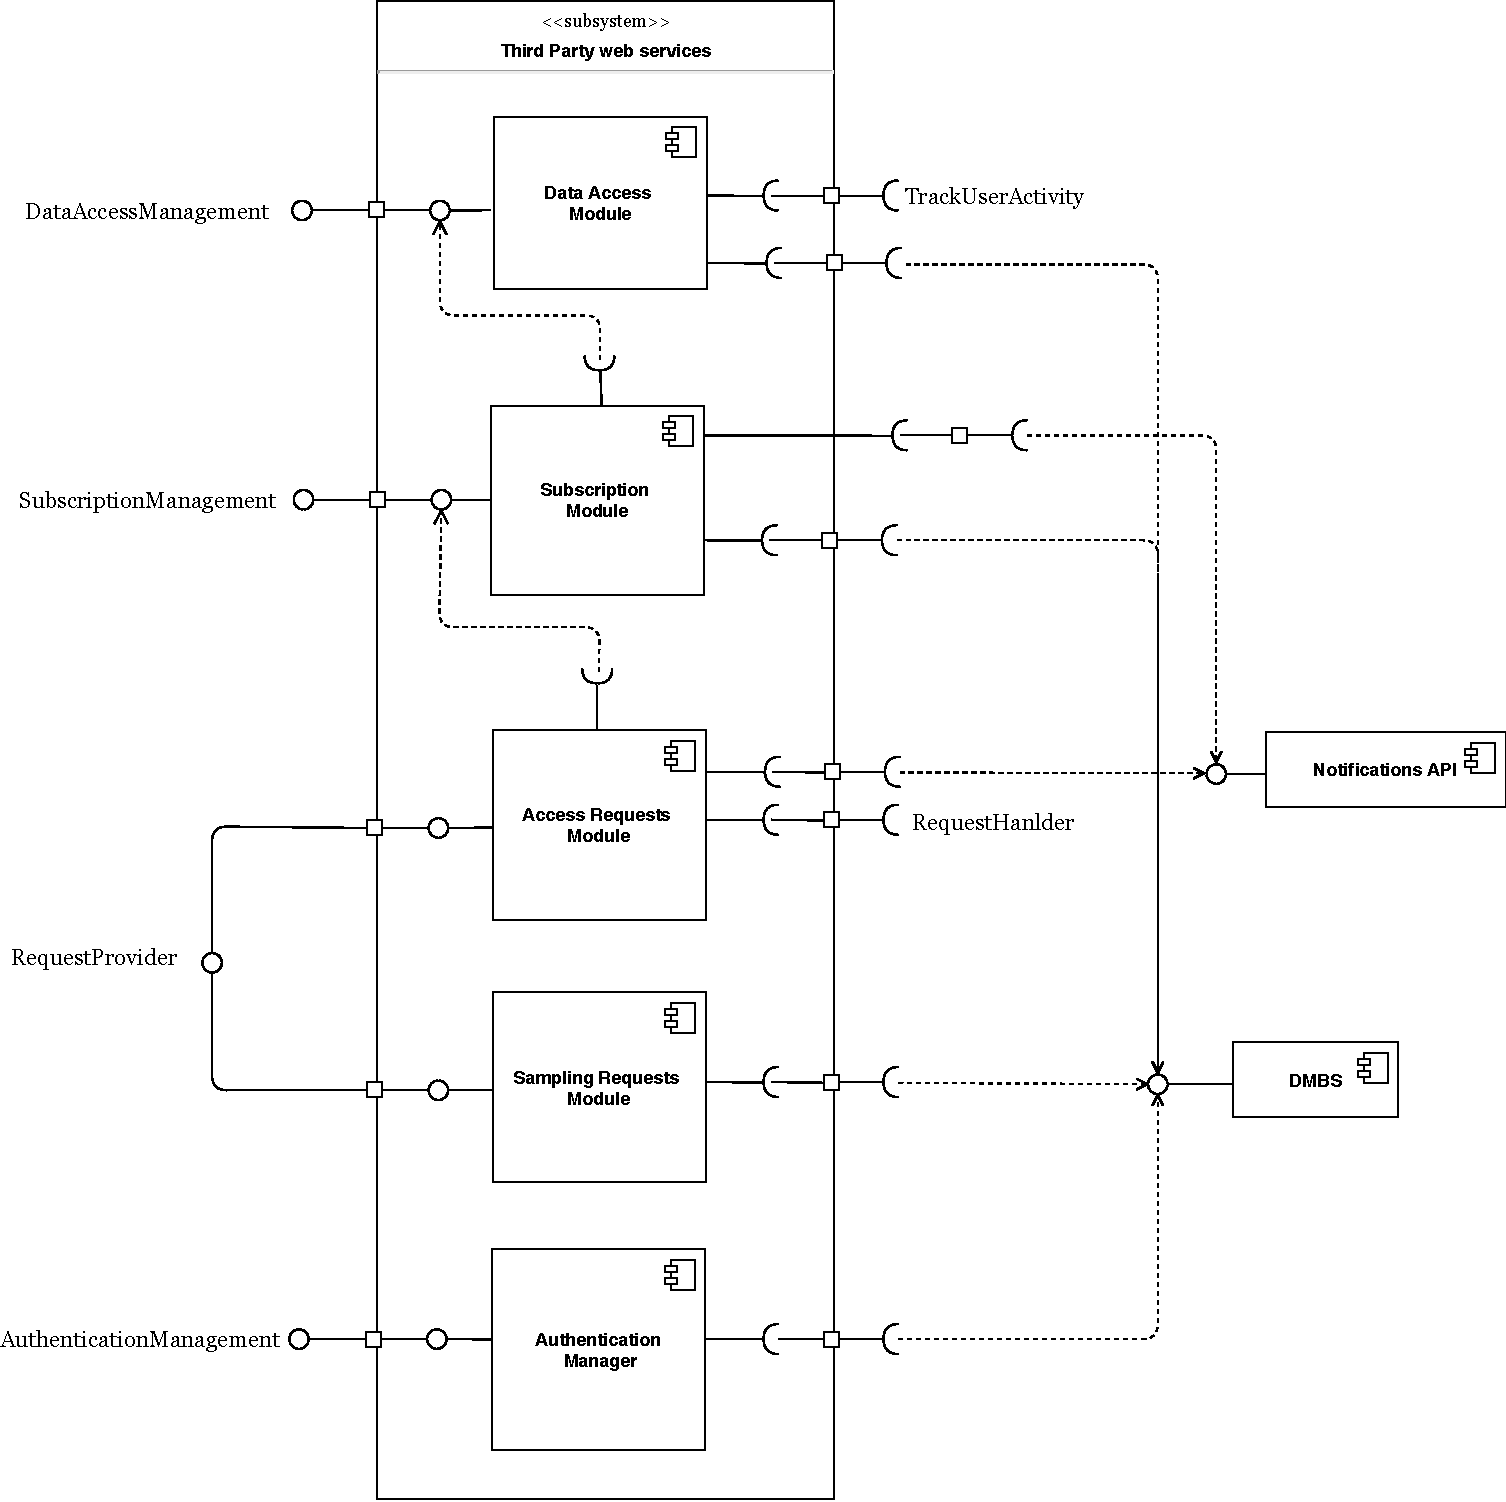
\includegraphics[height=1.0\linewidth]{images/third_party_projection}
				\label{fig:third_party_projection}
			\end{figure}
			\newpage
			\subsubsection*{Module Functionalities}
				\begin{itemize}
					\item \texttt{Data Access Module}: it deals with accessing to user's data, in case of the specific third party has access to him/her.
					\item \texttt{Subscription Module}: this component is responsible for subscribing a third party to a specific user, after the access request has been accepted. If the operation terminates successfully it checks the existence of new data retrieved by the Data Access Module and notifies the involved third party, thanks to the Notifications API.
					\item \texttt{Individual Requests Module}: it provides the third party with an interface that allows it to search a user and to send data access request to that specific user.
					If a request is accepted, it also gives the possibility to the third party to subscribe to user's new data, interfacing with the Subscription Module.
					\item \texttt{Sampling Requests Module}: similar to the Access Requests Module, provides an interface to allow the third party retrieving anonymized information of a group of users.
					\item \texttt{Authentication Manager Module}: this module provides all functionalities concerning with the registration and login of a third party to the system.
				\end{itemize}
			
		\newpage
		\subsection{Component Interfaces}
			\begin{figure}[H]
				\centering
				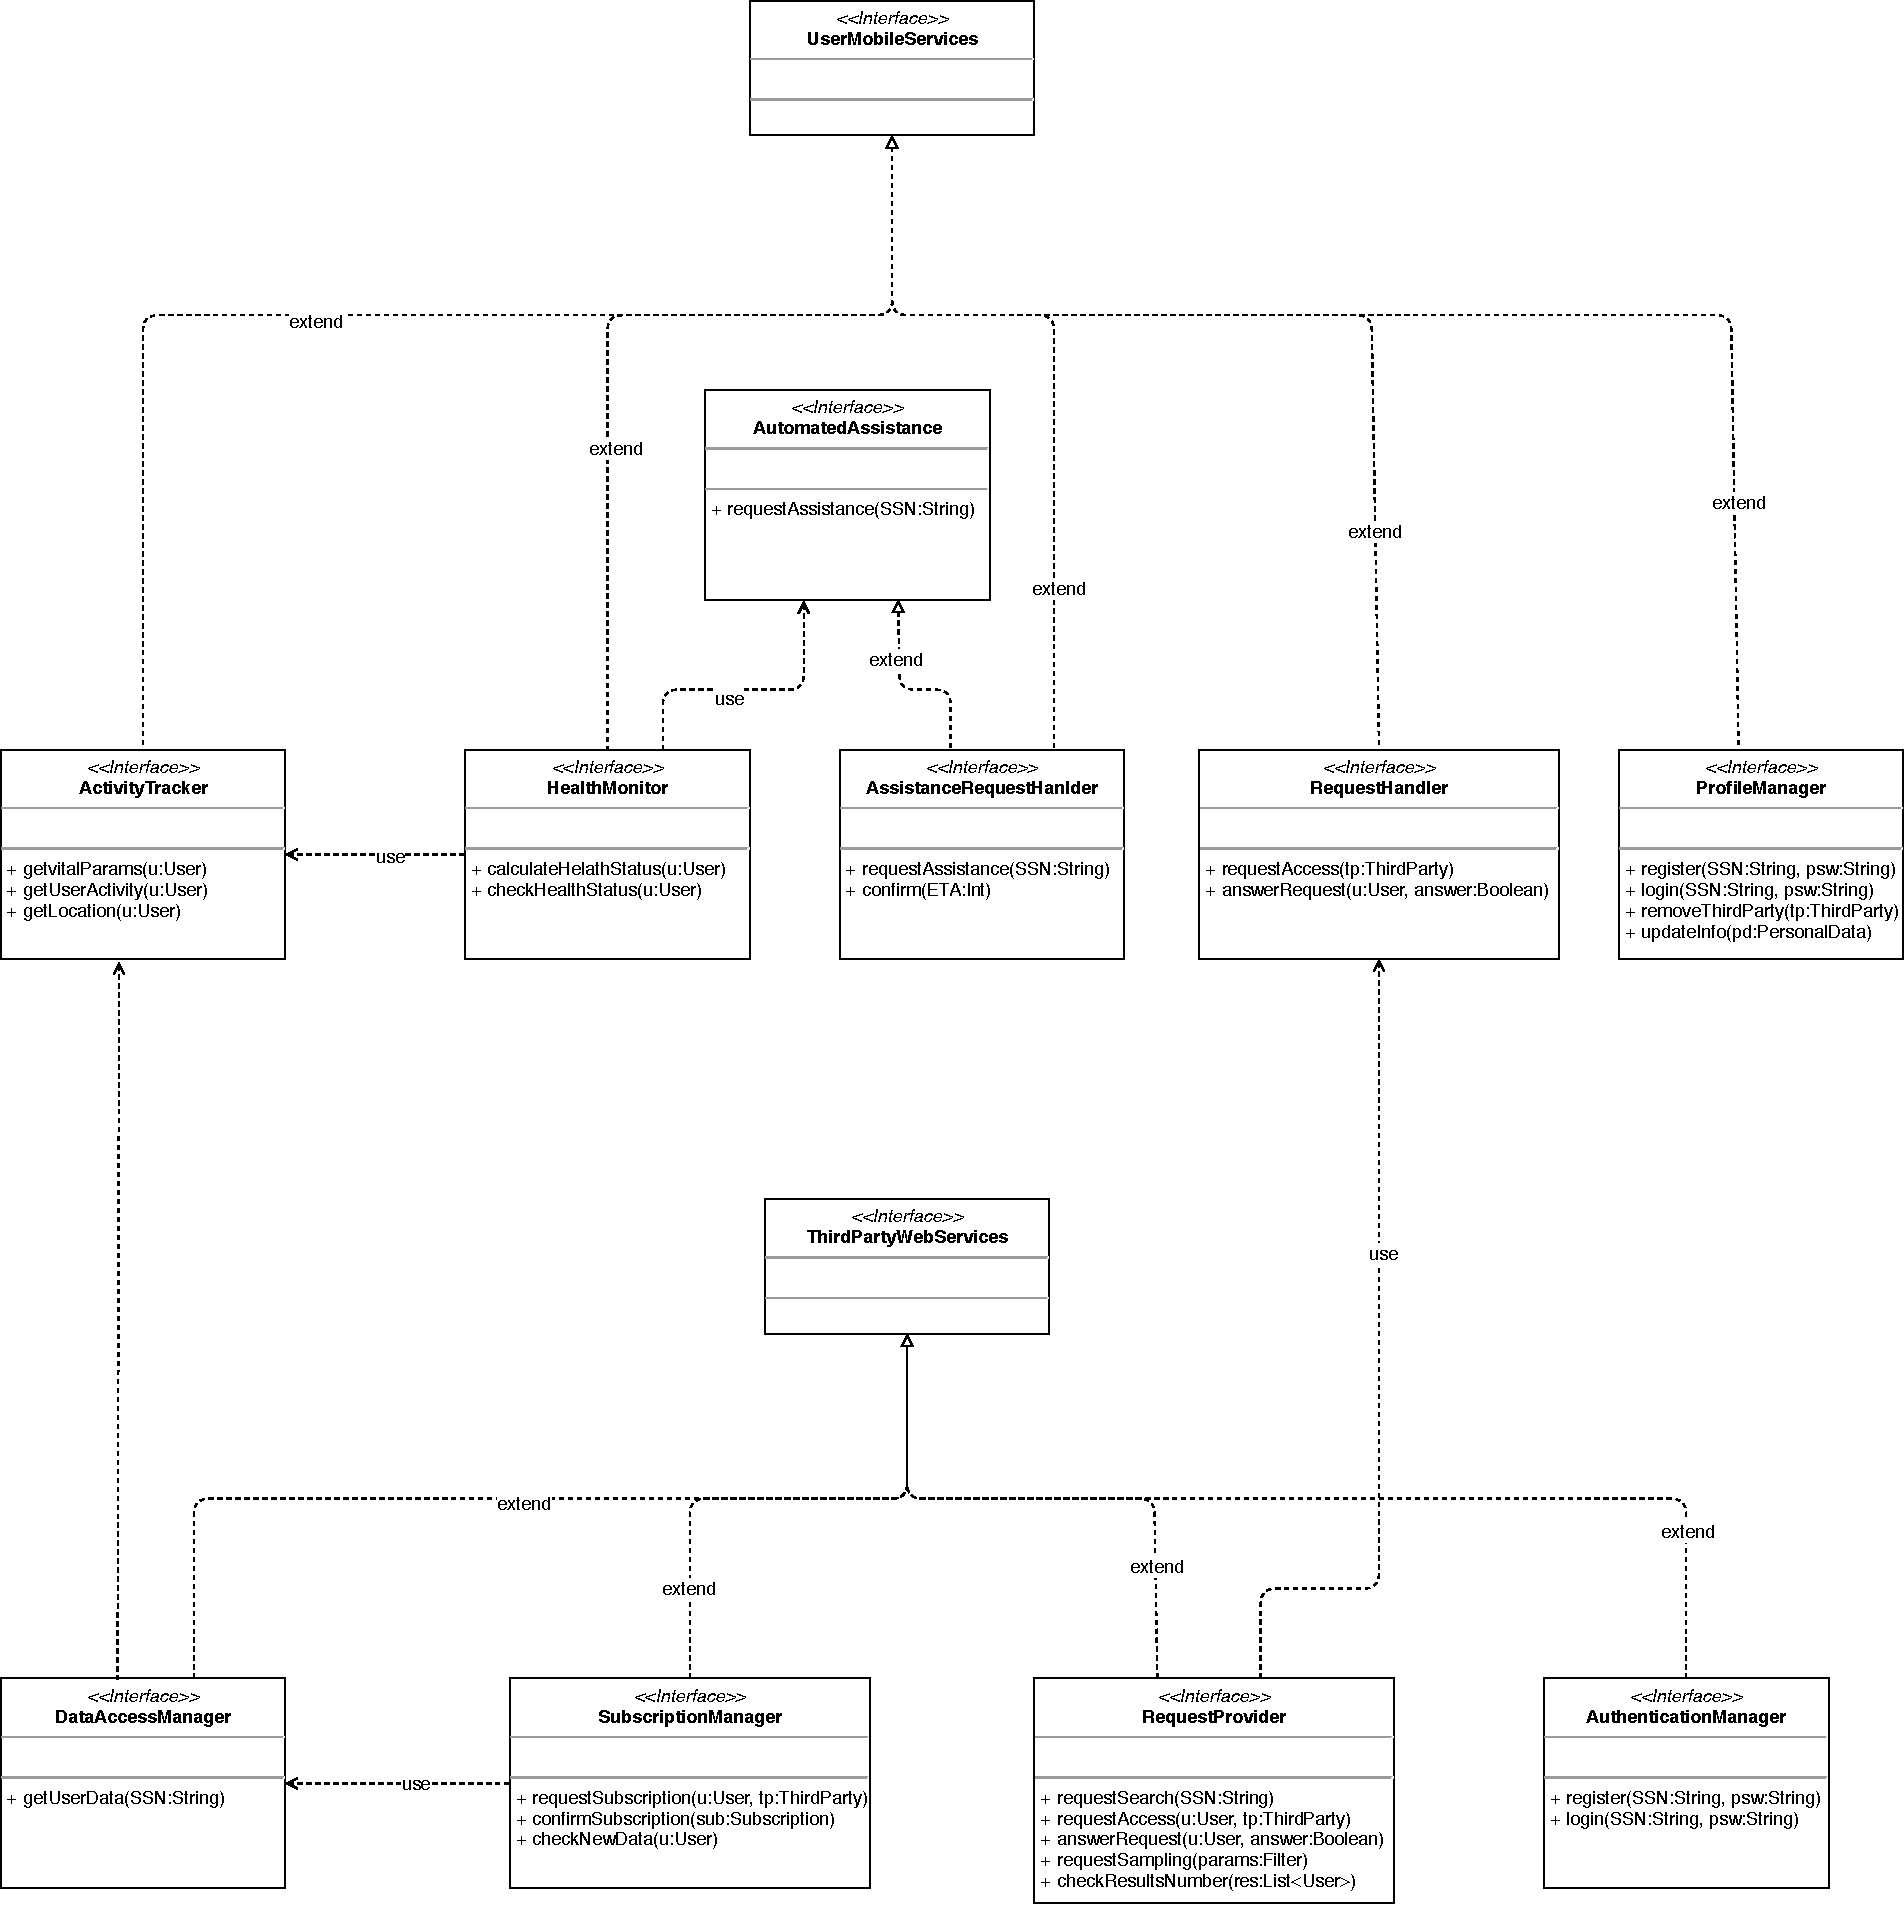
\includegraphics[height=1.2\linewidth]{images/comp_interfaces}
				\caption{Component interfaces and their interactions.}
				\label{fig:comp_interfaces}
			\end{figure}
			\newpage
			\subsubsection{External Interfaces}
			TrackMe will make use of some Application Programming Interfaces to simplify the implementation, since these components are largely used and compatible with the majority of the devices currently on the market:
			\begin{itemize}
				\item \texttt{Maps API} to have a visual representation of user location and to get it in critical moments, such as AutomatedSOS requests to the Ambulance Dispatching System. For our purpose the Google Maps API is perfectly suitable, since it can be embedded in both Android and iOS applications.
				\item \texttt{Sensors API} to read raw sensor data in real time. It allows listing the available sensors on the device on which te application is running and registering a listener on specific sensors to retrieve data automatically. For the Android system we selected the Google Sensors API and for iOS the native CoreMotion and HealthKit libraries.
				\item \texttt{Notifications API}: this lets applications send information to a user even if the app is idle or in the background. In the case if Android the app will use the Google Notifications API, while for iOS the standard library will be used.
				\item \texttt{Ambulance Dispatching System API} to perform assistance requests. Actually it could be an automatic phone call to the ambulance contact center, during which an algorithm communicates all relevant data to the interlocutor (e.g. name, age, location etc.).
				\item \texttt{Database API} to support multiple database servers easily, to provide a structured interface for the dynamic construction of queries and to enforce security checks.
				\item \texttt{SMS API} to enable code to send short messages via a SMS Service, such as during the registration process.
			\end{itemize}
			
		\newpage
		\subsection{Model and Database Structure}
			In this section, a description of the model structure is given. \\
			The following UML Class Diagram is used to map the model components to their correspondant database tables. Moreover, we give an idea of what types of data are needed and what attributes are related to the described data structures.
			\begin{figure}[H]
				\centering
				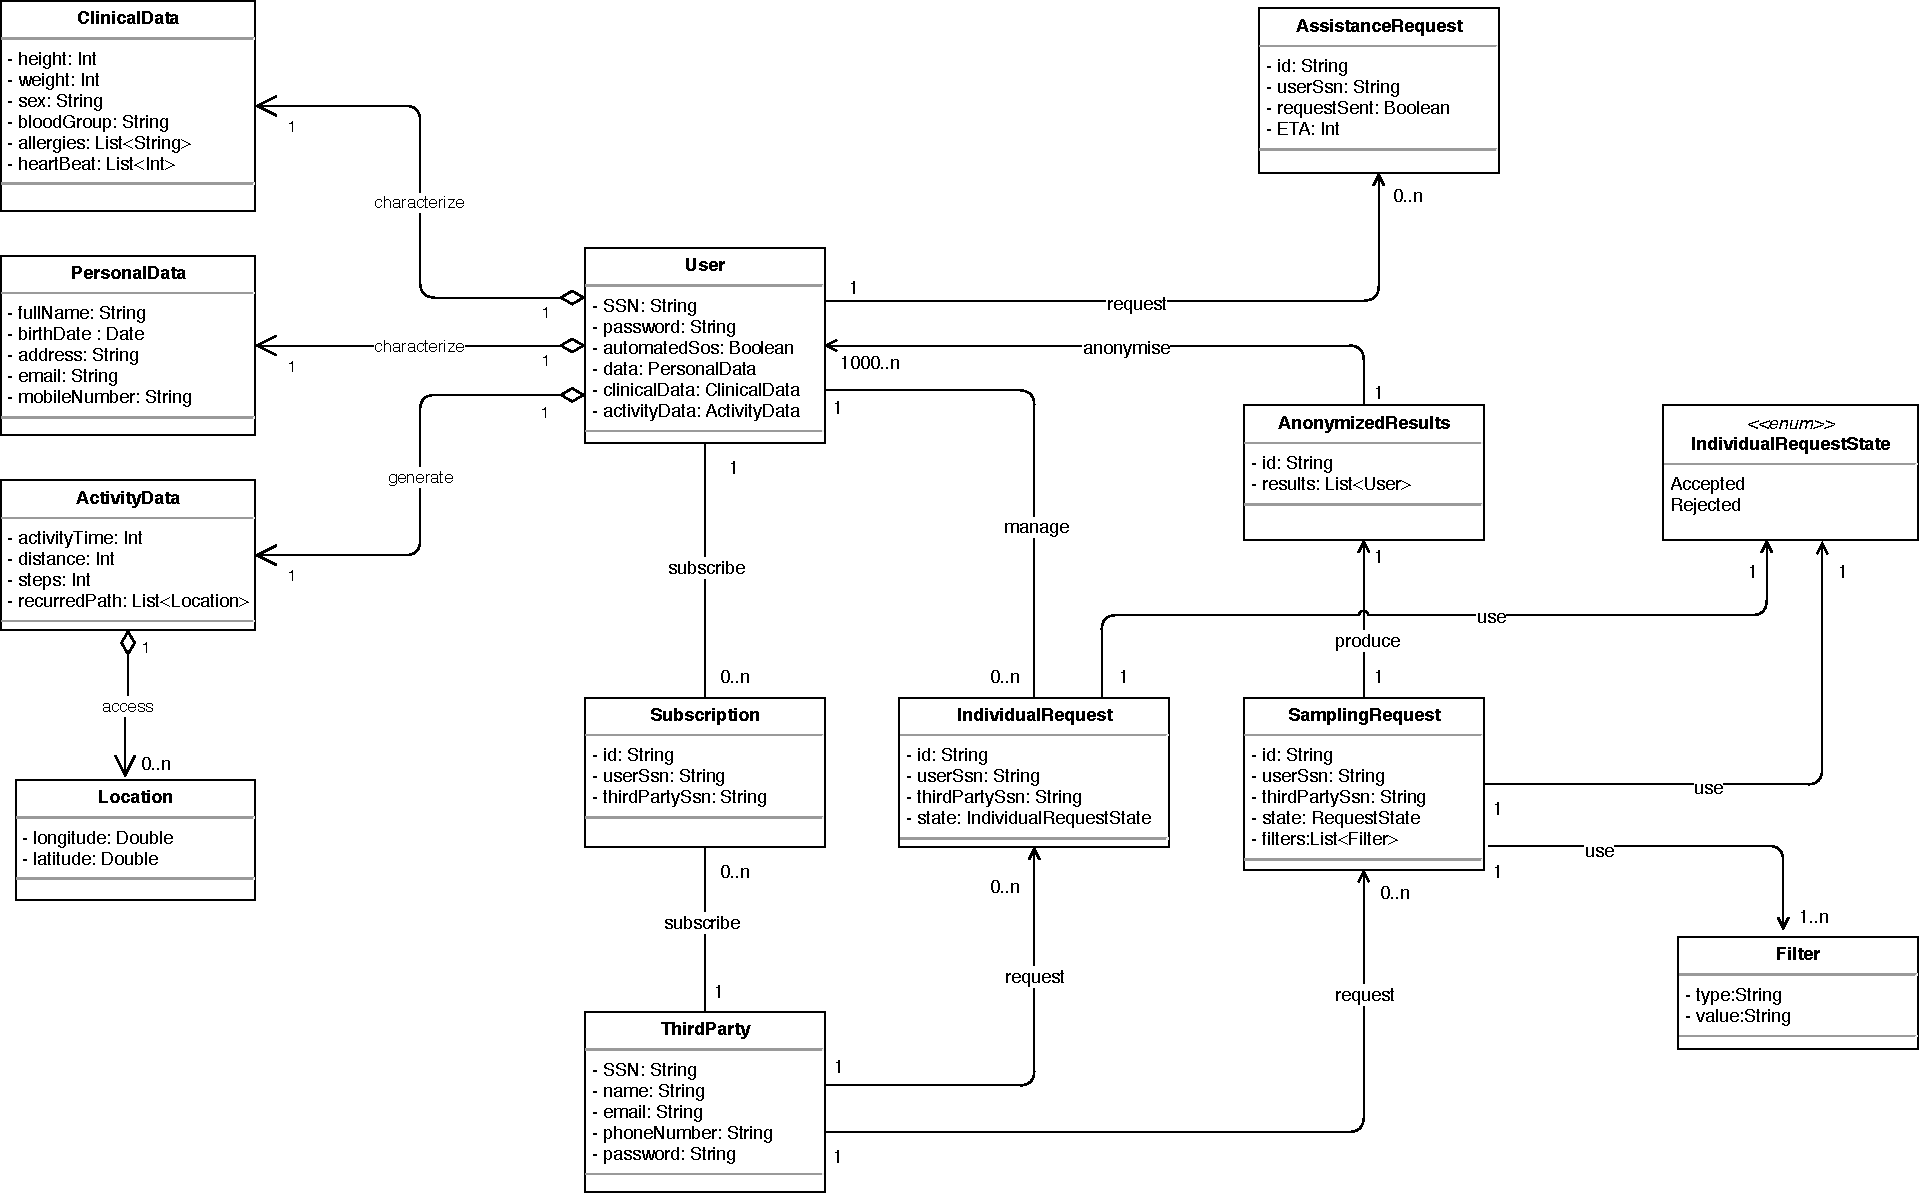
\includegraphics[width=1.2\linewidth]{images/UML}
				\caption{UML Class Diagram for database structure.}
				\label{fig:UML}
			\end{figure}
		
		\newpage
		\subsection{Deployment View}
				For the deployment of the system, we opted for a 4-tier architecture composed as follows:
				\begin{itemize}
					\item \textbf{Tier 1}\\
					This tier is composed by the Client (implemented as a Thin Client), that includes the Web App (run by a web browser) and the Mobile Application (run by smartphones and smartwatches). 
					\item \textbf{Tier 2}\\
					This tier is composed by the Web Server, whose main functionality is to store, process static content and deliver web pages to the Clients. For this reason, we opted for NGINX, that guarantees better perfomances for static content processing. It can be also configured as a load balancer, in order to better handle multiple connections.
						\begin{figure}[H]
							\centering
							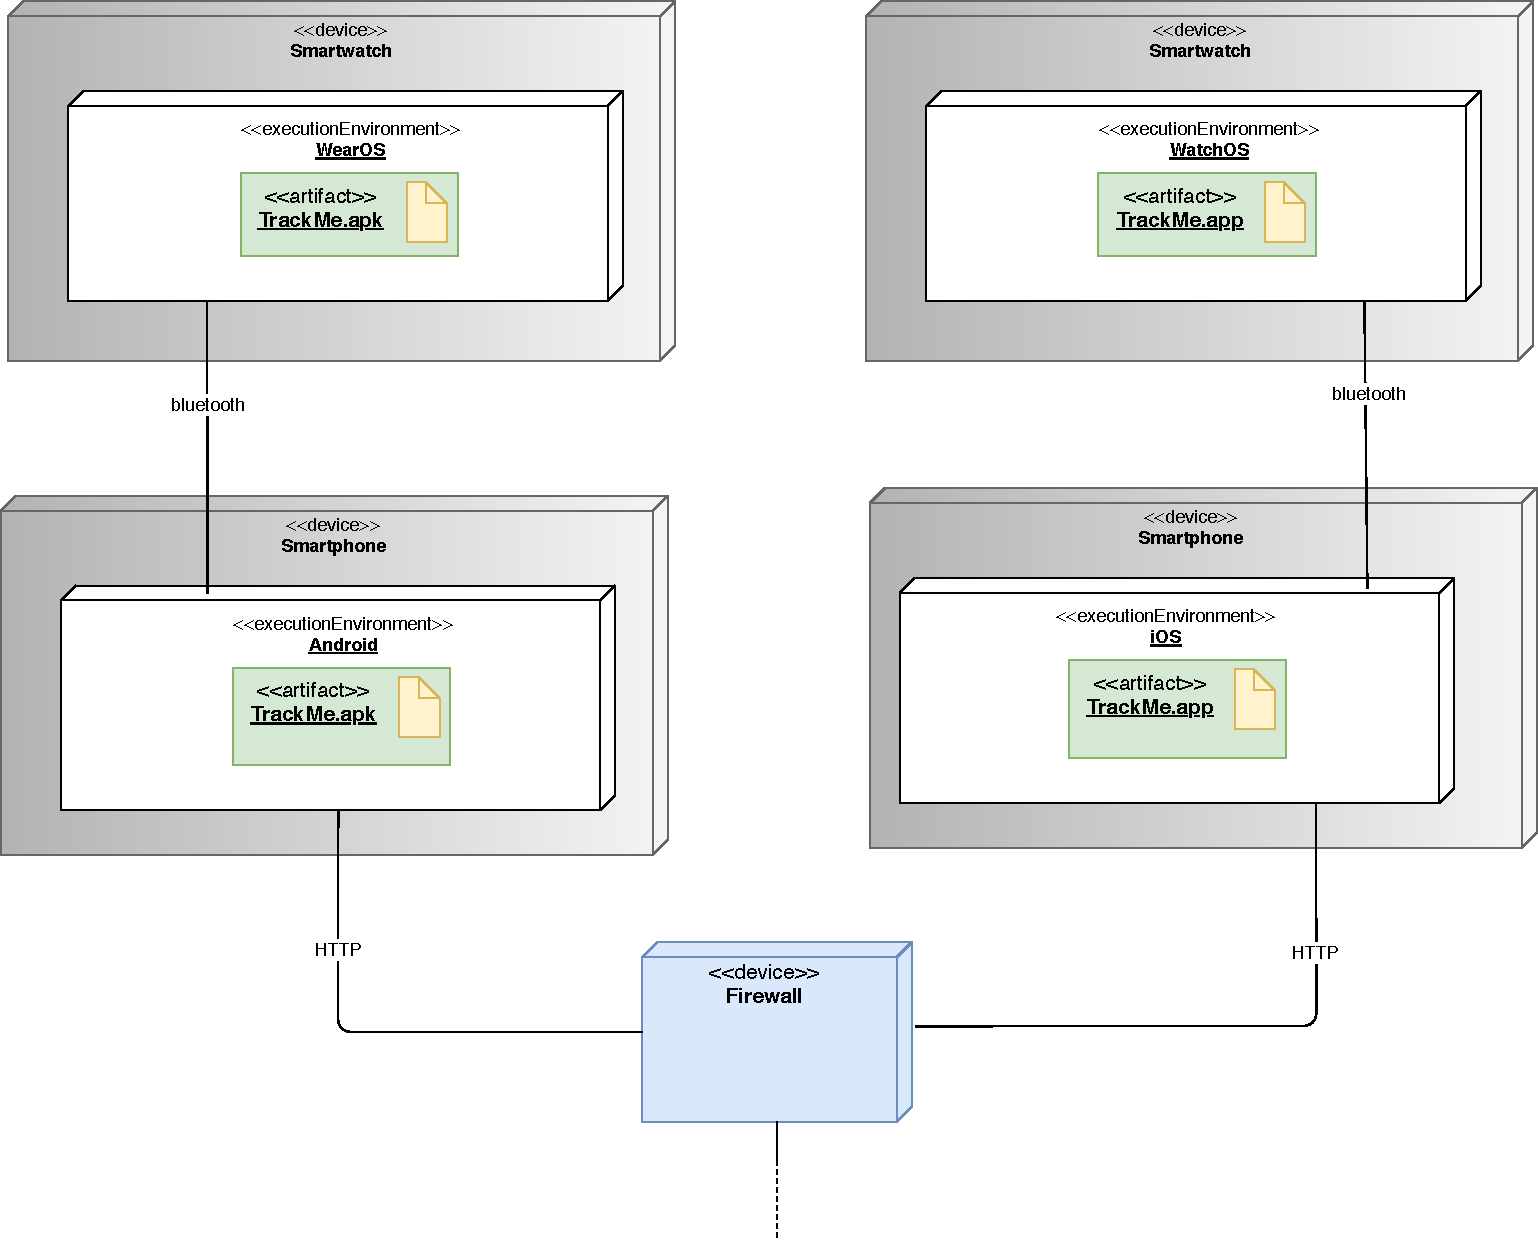
\includegraphics[width=0.8\linewidth]{images/mobile_artifacts}
							\caption{Deployment View for Mobile Application (Tier 1).}
							\label{fig:mobile_artifacts}
						\end{figure}
						\begin{figure}[H]
							\centering
							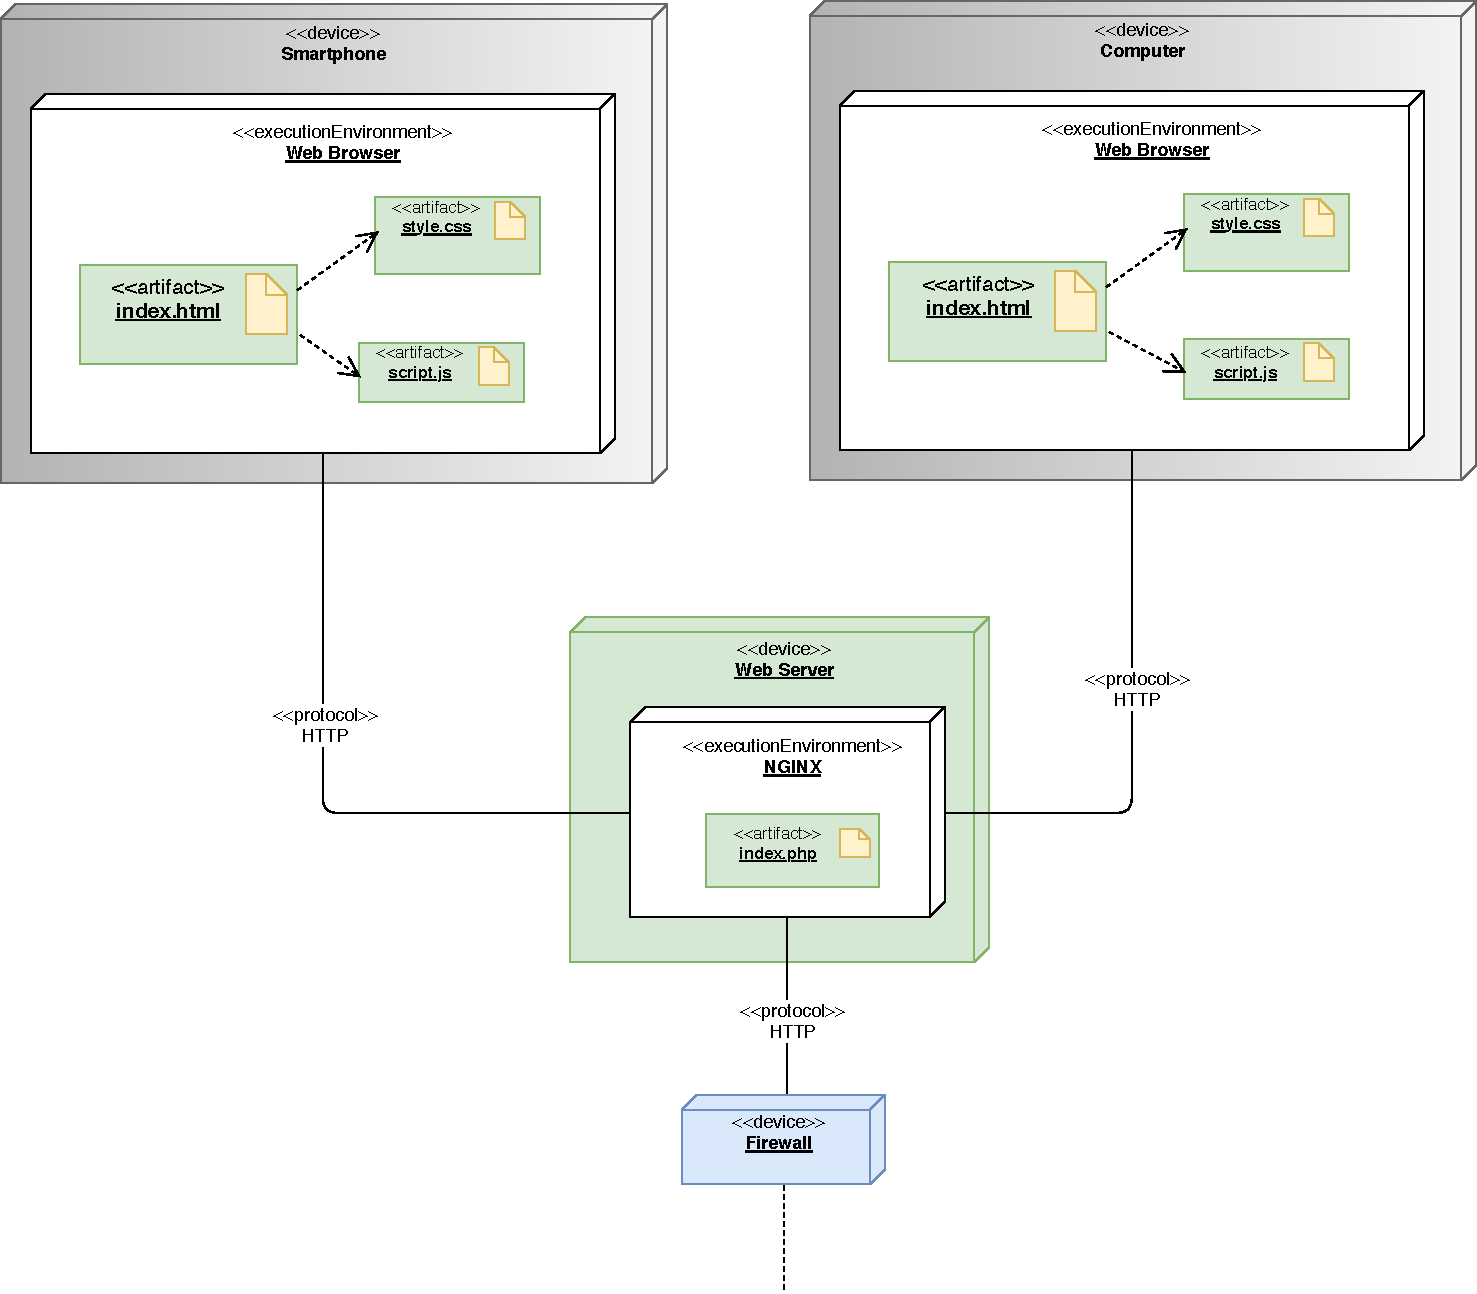
\includegraphics[width=0.6\linewidth]{images/web_browser_artifacts}
							\caption{Deployment View for Web Browser clients and Web Server (Tier 1 and 2).}
							\label{fig:web_browser_artifacts}
						\end{figure}
					\item \textbf{Tier 3}\\
					This tier corresponds to the Application Server, that provides both facilities to create web applications and a server environment to run them. We opted for WildFly (v. 12.0.0 or recent versions - previously JBoss) since it fully implements all Java EE specifications.
						\begin{figure}[H]
							\centering
							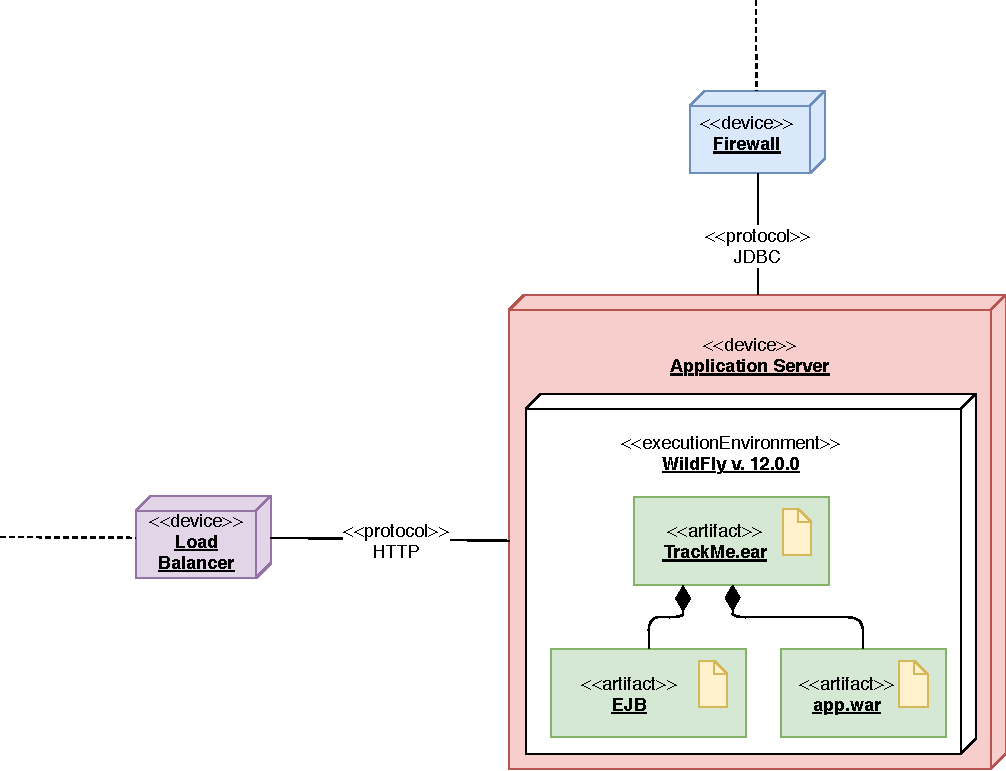
\includegraphics[width=0.7\linewidth]{images/app_server_artifacts}
							\caption{Deployment View for Application Server (Tier 3).}
							\label{fig:app_server_artifacts}
						\end{figure}
					\item \textbf{Tier 4}\\
					This tier corresponds to the Database Server on which the DBMS is running. We opted for MySQL (v. 8.0.12) since it is one of the most secure and reliable database management system used in popular web applications and guarantees scalability and high performance. \\ \\
				\end{itemize}
			The following diagram represents how the previously described tiers are assembled:
			\begin{figure}[H]
				\centering
				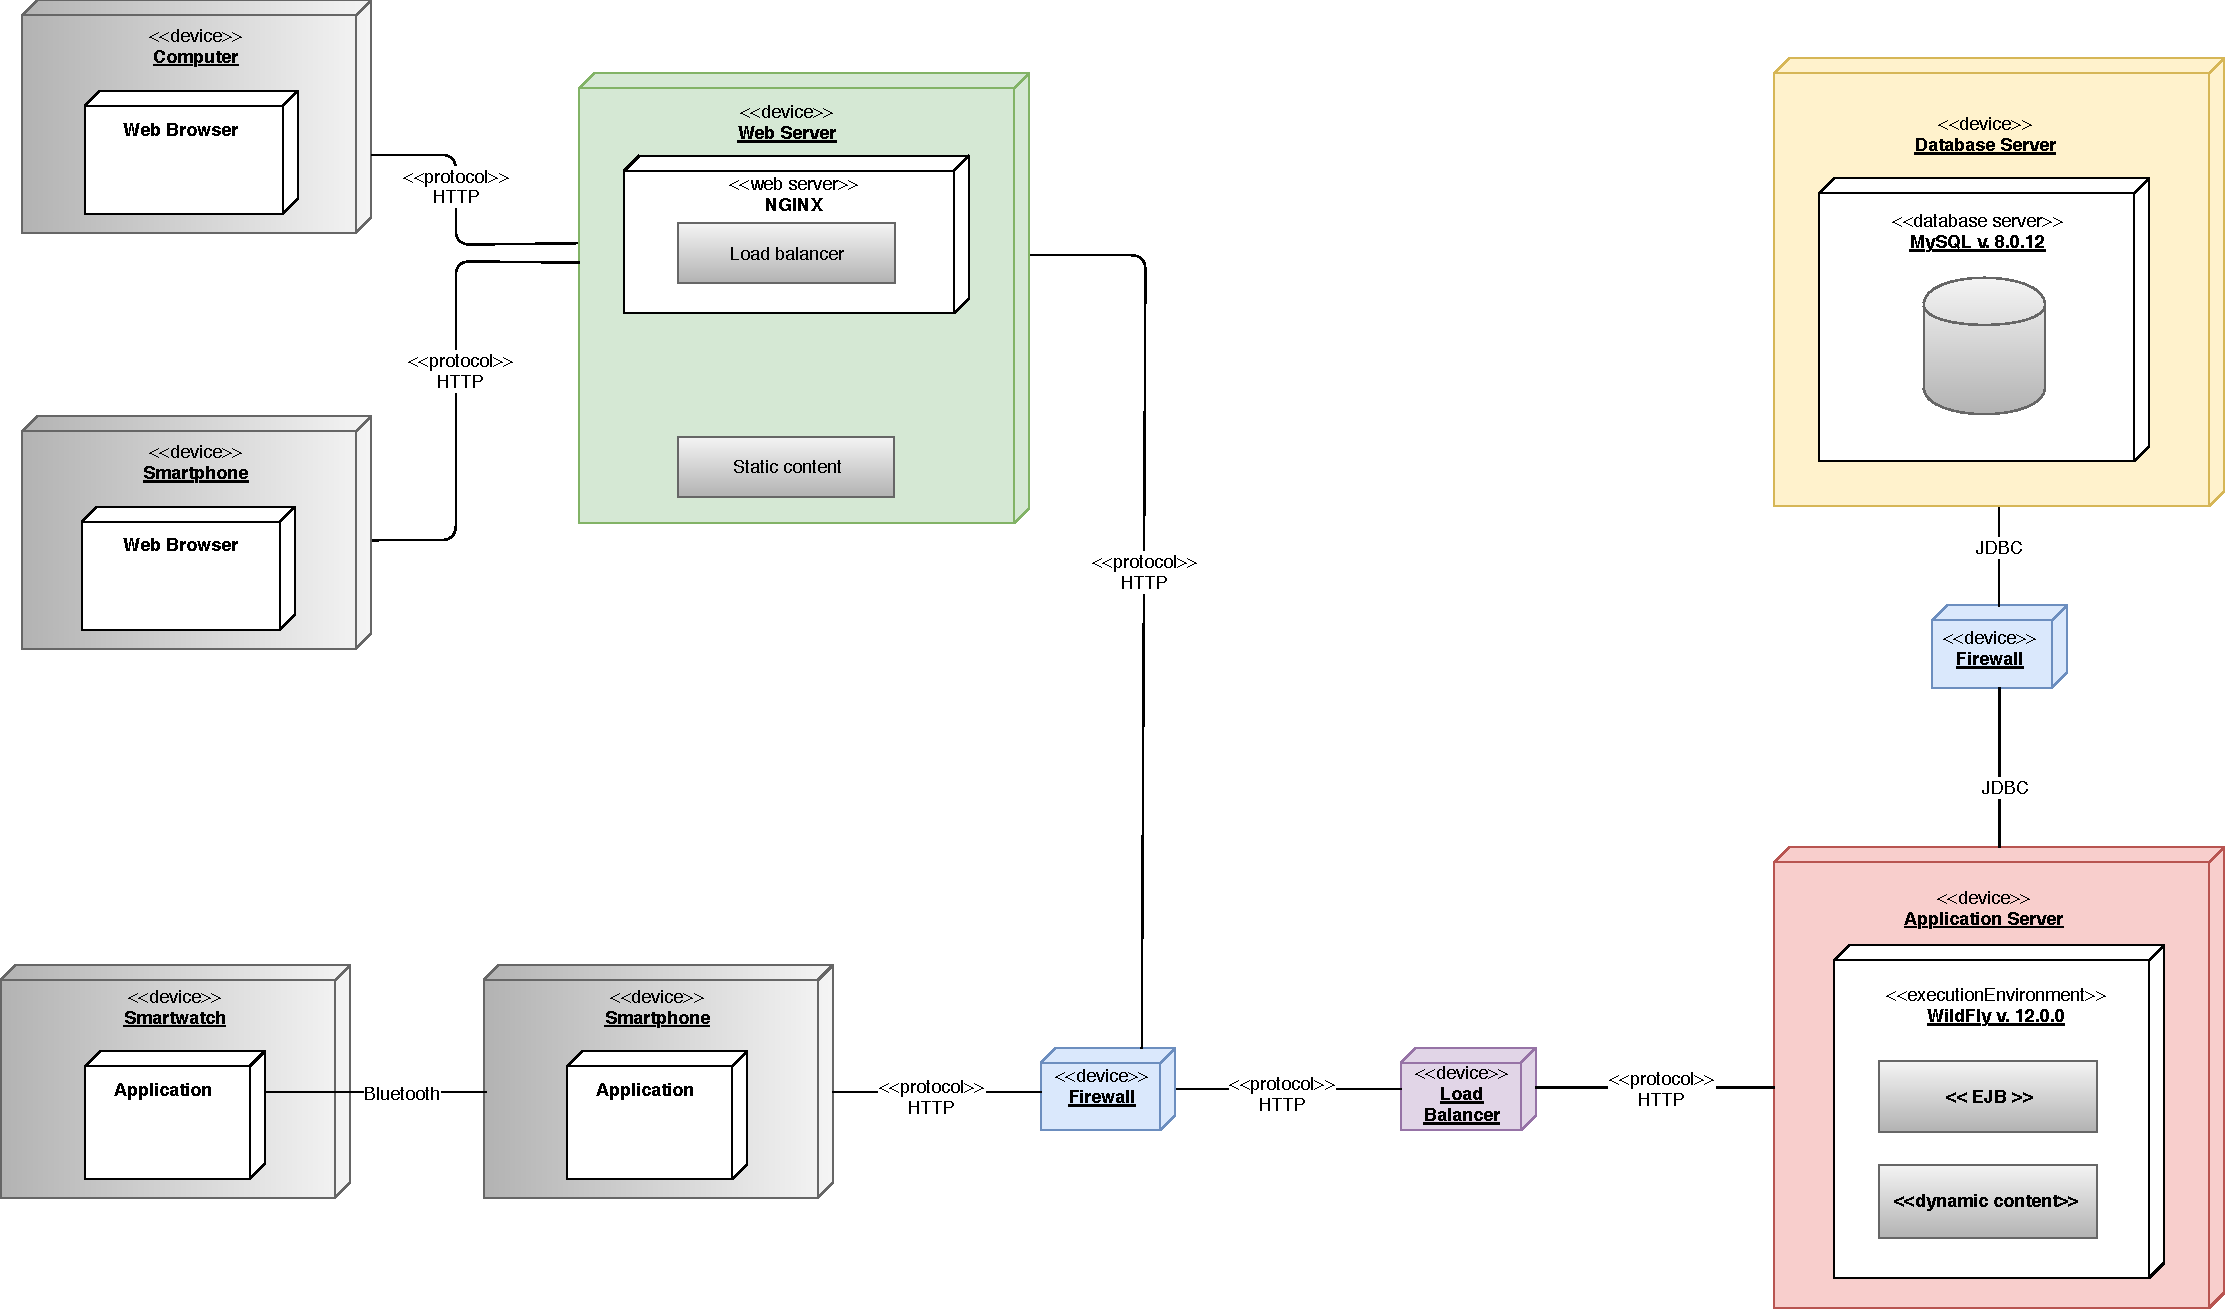
\includegraphics[width=1.2\linewidth]{images/deployment_diagram}
				\caption{Deployment View Diagram (entire system).}
				\label{fig:deployment_diagram}
			\end{figure}
		
		\newpage
		\subsection{Runtime View}
			\subsubsection{On-Demand Assistance Request}
					\begin{figure}[H]
					\centering
					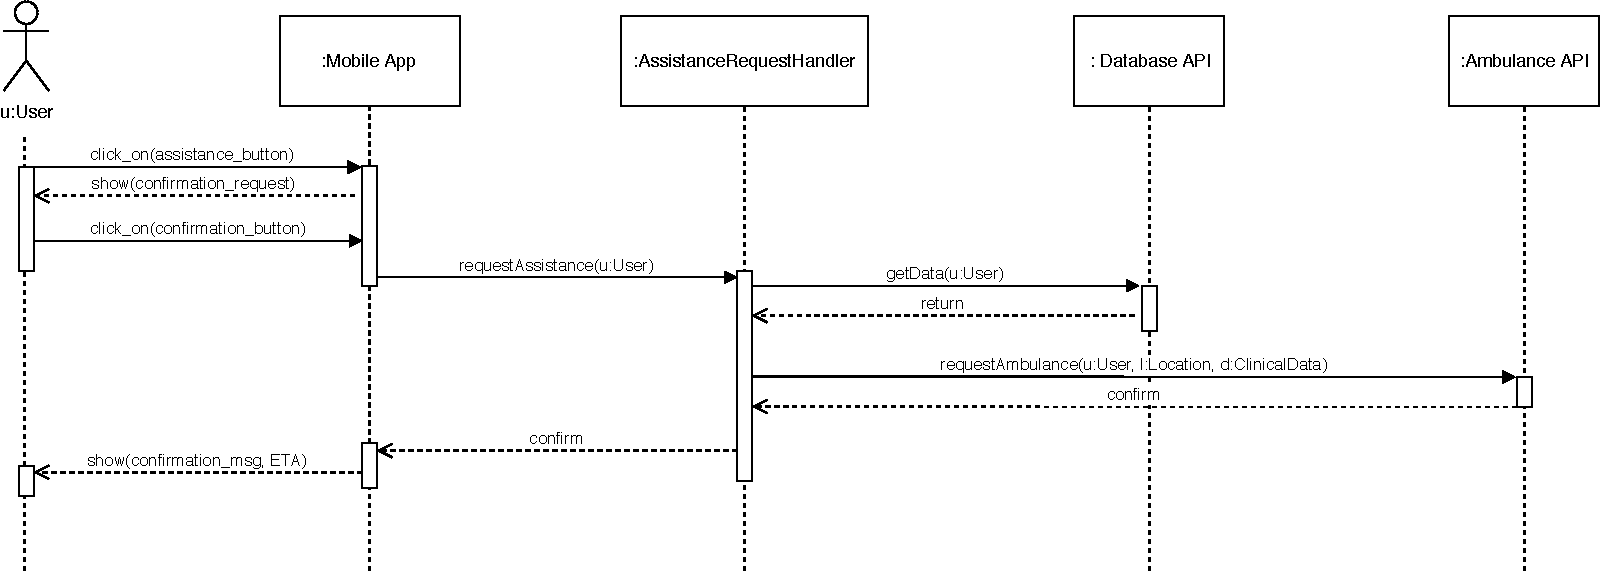
\includegraphics[width=1.0\linewidth]{images/ass_request_sequence}
					\label{fig:ass_request_sequence}
				\end{figure}
				In this sequence diagram the on-demand assistance request process is shown. The main component of this process is the AssistanceRequestHandler. The process begins when a User clicks on the assistance button and the Mobile App notifies the AssistanceRequestHandler which in turn queries the Database. From the Database, information about the user is retrievied and then forwarded to the Ambulance API, where it is processed in order to send an ambulance to assist the User. A confirmation message is returned in first place to the AssistanceRequestHandler and then to the Mobile App and with a show() method the UI is updated.
				\newpage
				\subsubsection{Automated Assistance Request}
				\begin{figure}[H]
					\centering
					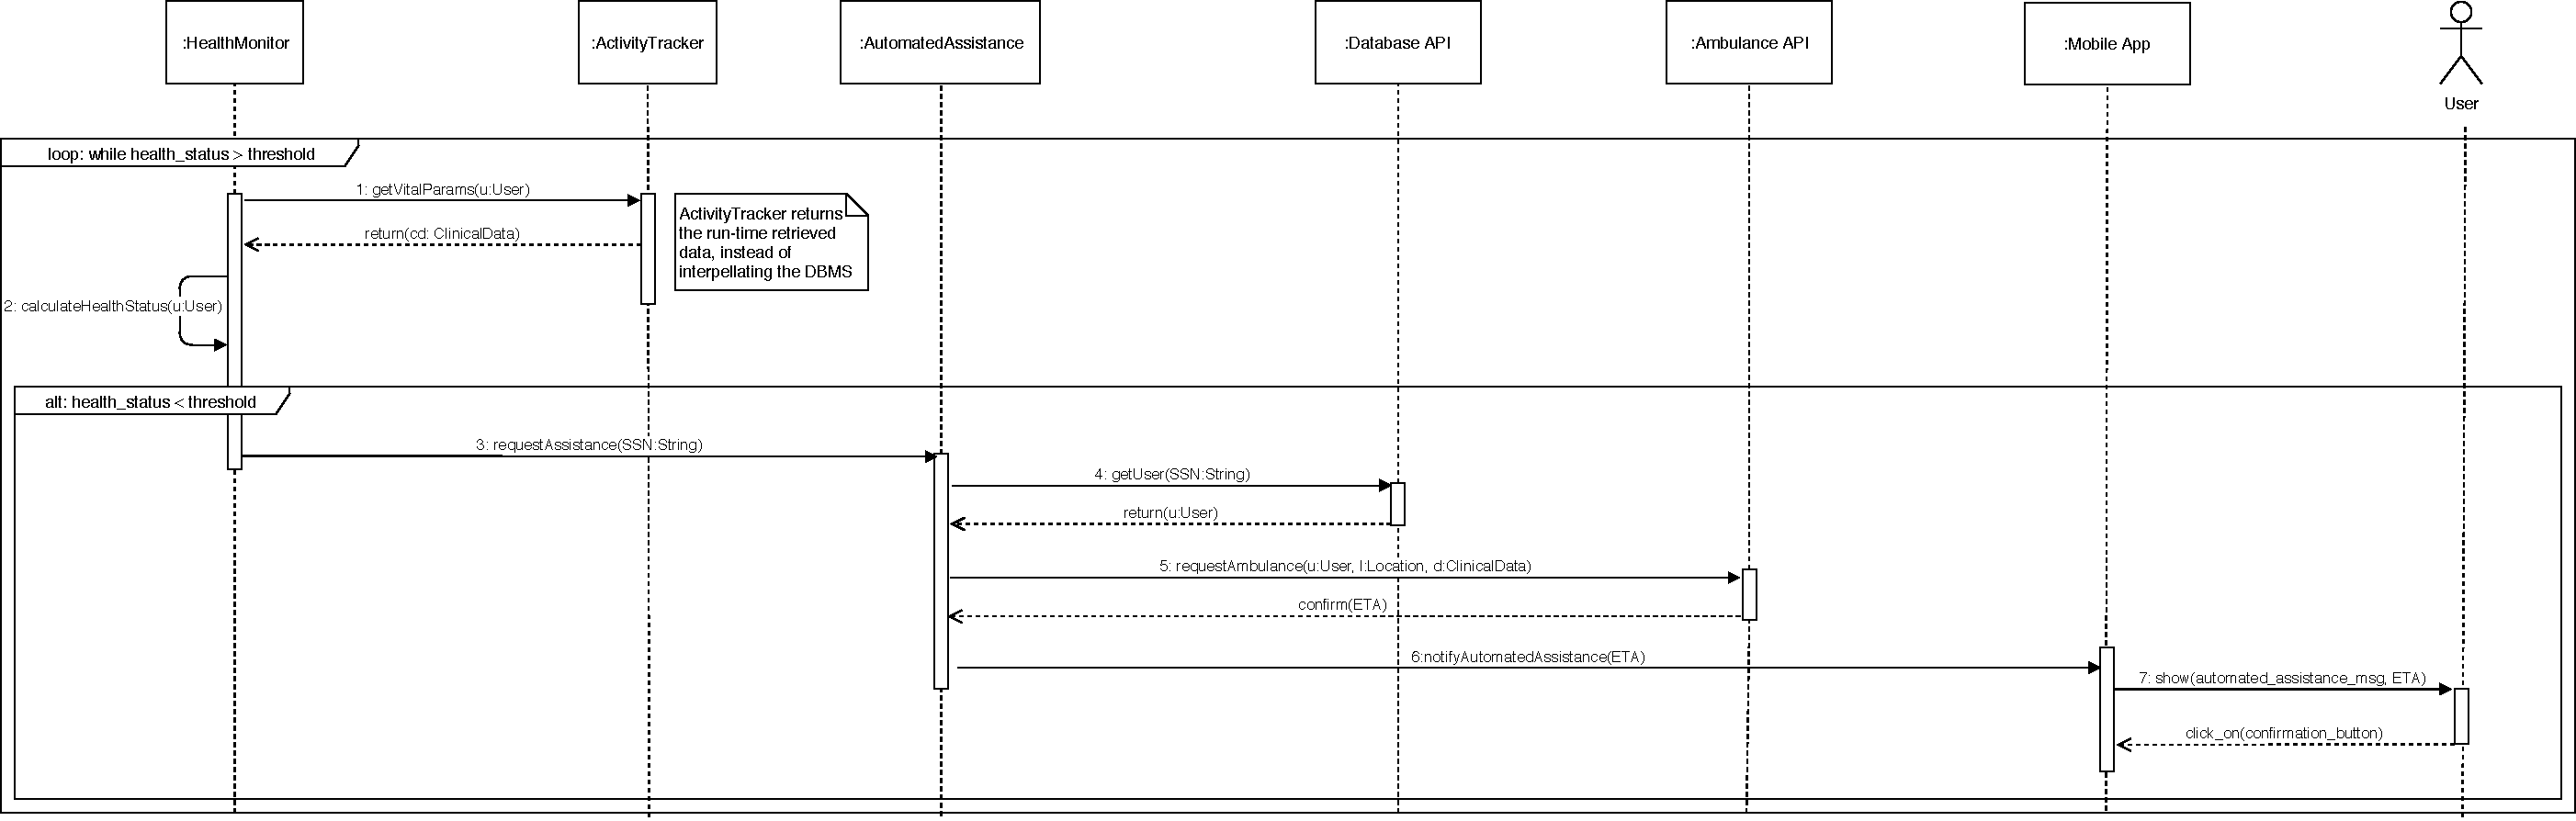
\includegraphics[width=1.0\linewidth]{images/automated_request_sequence}
					\label{fig:automated_request_sequence}
				\end{figure}
				In this sequence diagram the automated assistance request process is shown. The main components of this process are the AutomatedAssistance interface and the HealthMonnitor. The process in the HealthMonitor where it loops calculating health status of a generic User and retrieves vital parameter from the Activity Tracker. When some parameters are below a fixed threshold, a request assistance is forwarded to the AutomatedAssistance interfaces which in turn retrieves information from the database and then forwards it to the Ambulance API, where it is processed to send an ambulance to assist the User. A notification is sent afterwards to the User, updating the UI.
				\newpage
				\subsubsection{Data Access Request}
				\begin{figure}[H]
					\centering
					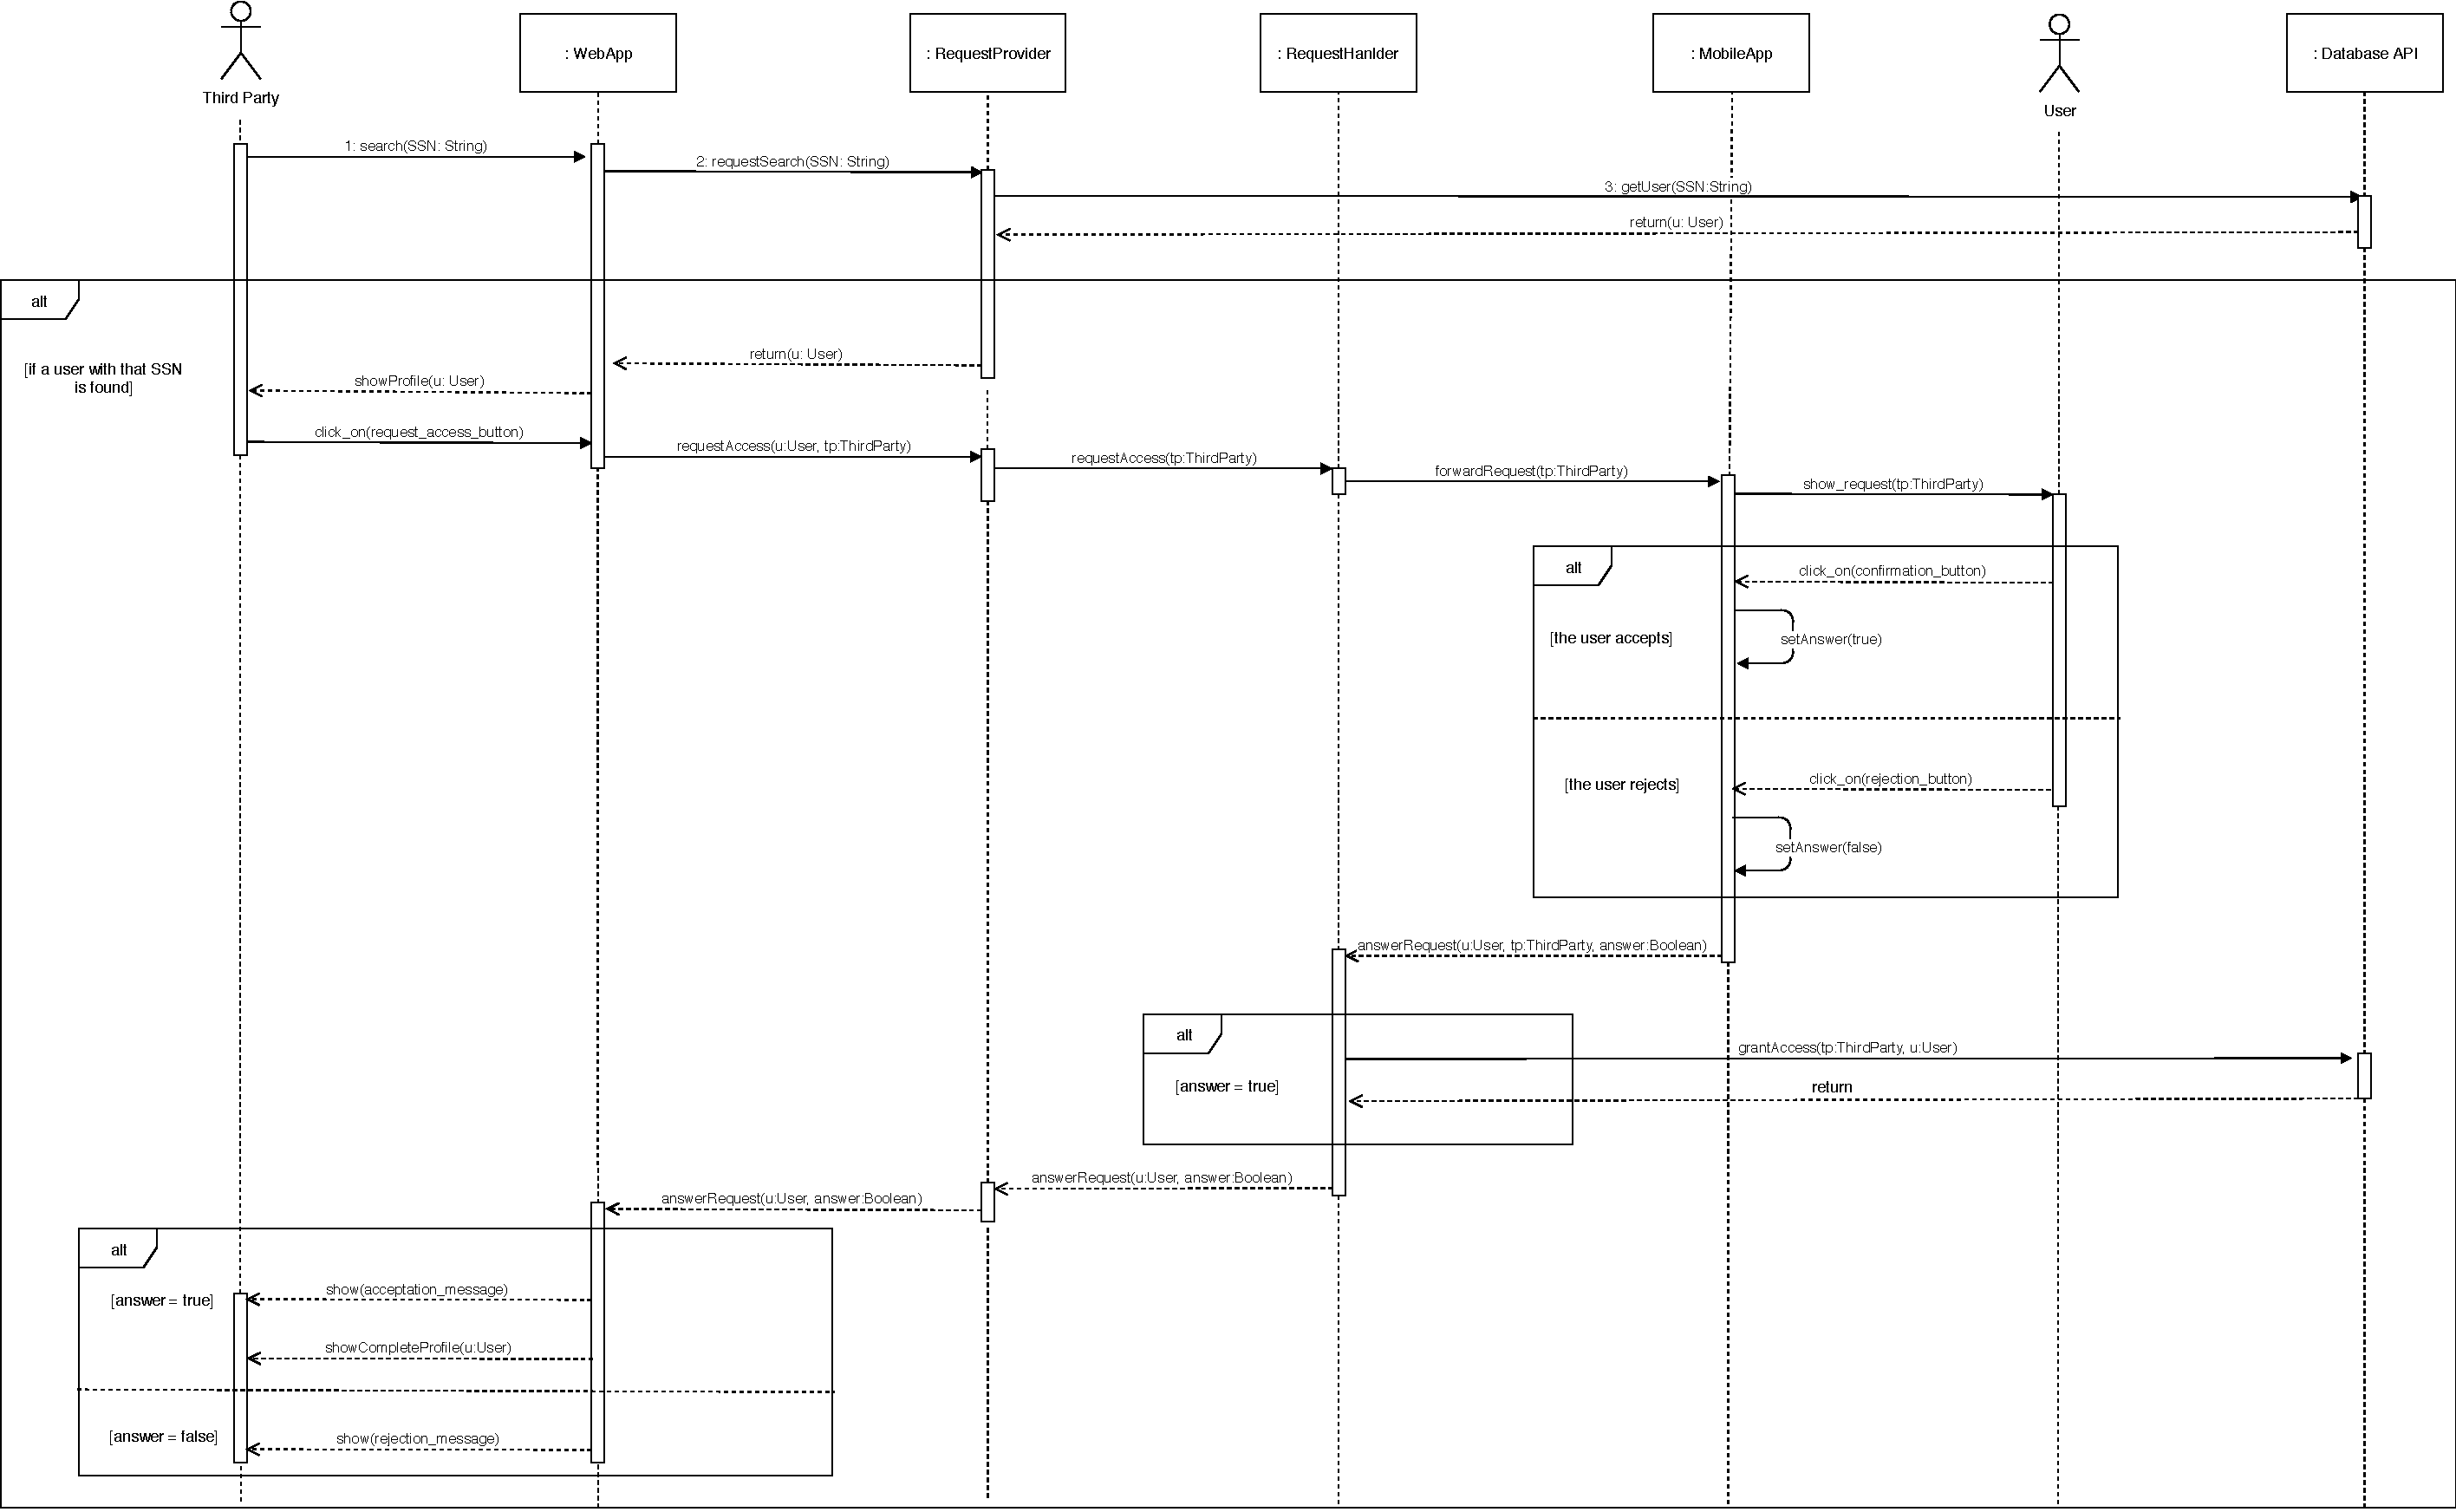
\includegraphics[width=1.0\linewidth]{images/access_request_sequence}
					\label{fig:access_request_sequence}
				\end{figure}
				In this sequence diagram the data access request process is shown. The main components of this process are the RequestProvider and the RequestHandler. The process begins when a third party searches for a user throught the web app. A search request is sent to the RequestProvider that in turn retrieves information about the specific user from the database. If the User's SSN has been found in the database, his profile is returned to the third party which can in turn send a request to access his profile. Such request is forwarded in first place to the RequestProvider and then to the RequestHandler. When such request is sent, the User can either either accept it or refuse from the app, and then the answer is notified back to the third party, refreshing the web page either with a confirmation message and showing the user profile or with a rejection message.
				\newpage
				\subsubsection{Subscription to User's Data}
				\begin{figure}[H]
					\centering
					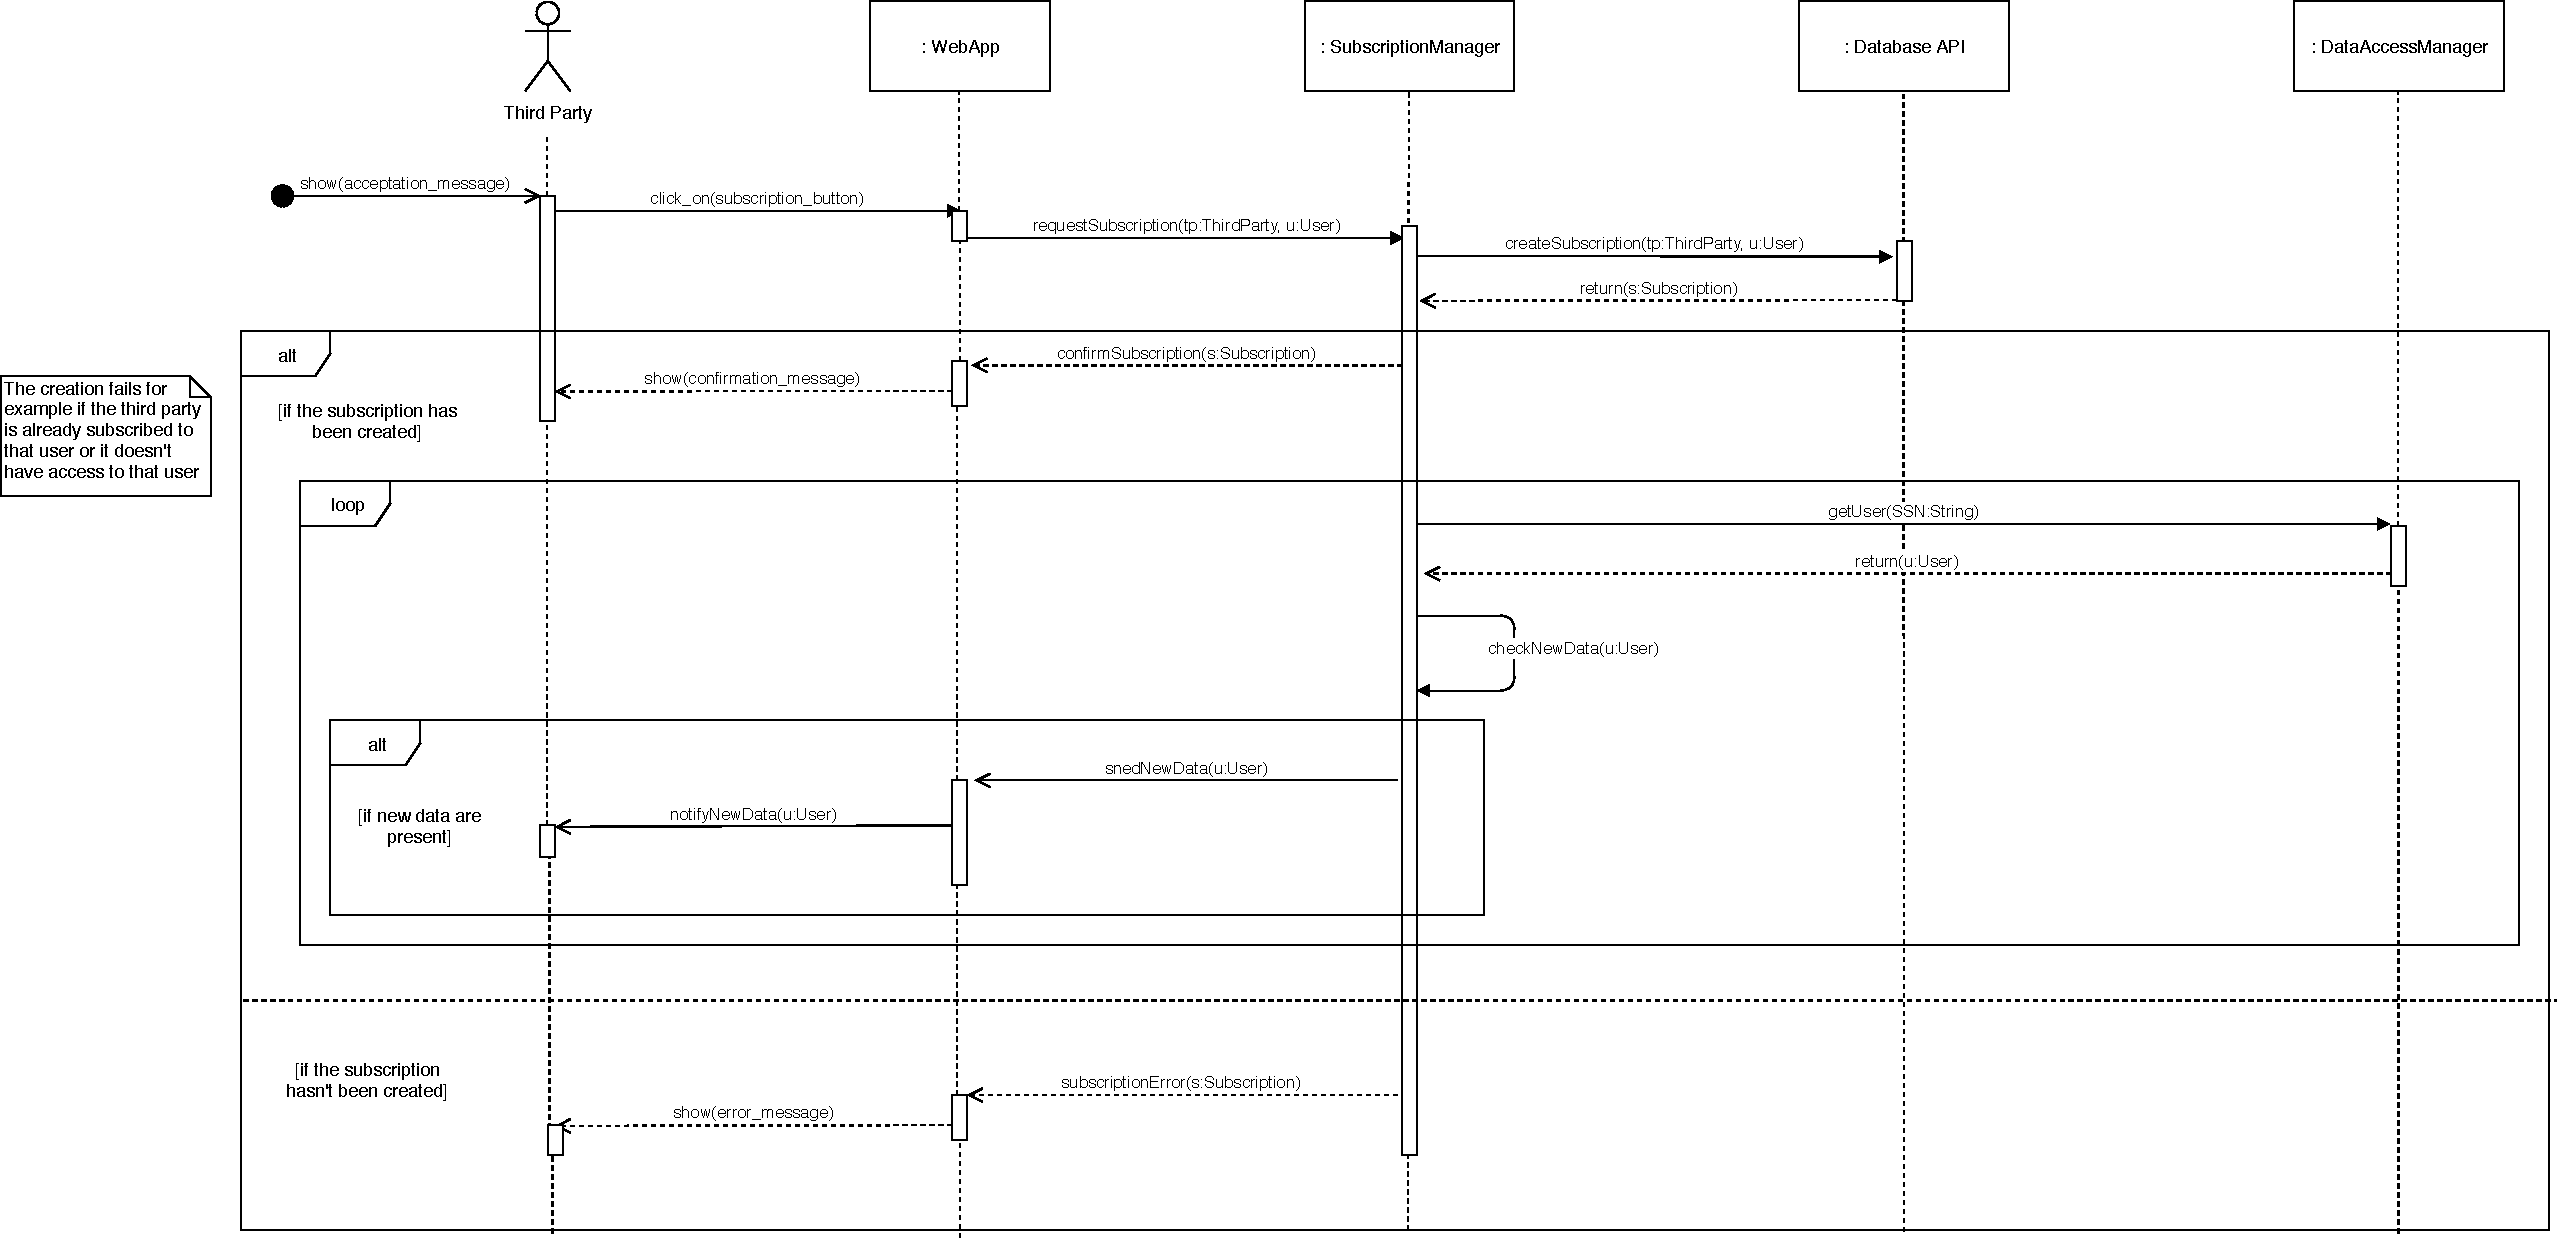
\includegraphics[width=1.0\linewidth]{images/subscription_sequence}
					\label{fig:subscription_sequence}
				\end{figure}
				In this sequence diagram the subscription to user's data process is shown. The main component of this process is the SubscriptionManager. This process is asynchronous and can begin if and only if a User has accepted the access to his/her profile from a third party. A third party, through the Web App, can click on the subscription button and a subscription request is notified to the SubscriptionManager which in turn creates a subscription and stores its information in the database. A confirmation message is returned afterwards to the Web App and a confirmation message is shown to the third party. From this point, whenever new data is generated, the system loops and retrieves it, refreshing the third party web app.
				\newpage 
				\subsection{Sampling Search}
				\begin{figure}[H]
					\centering
					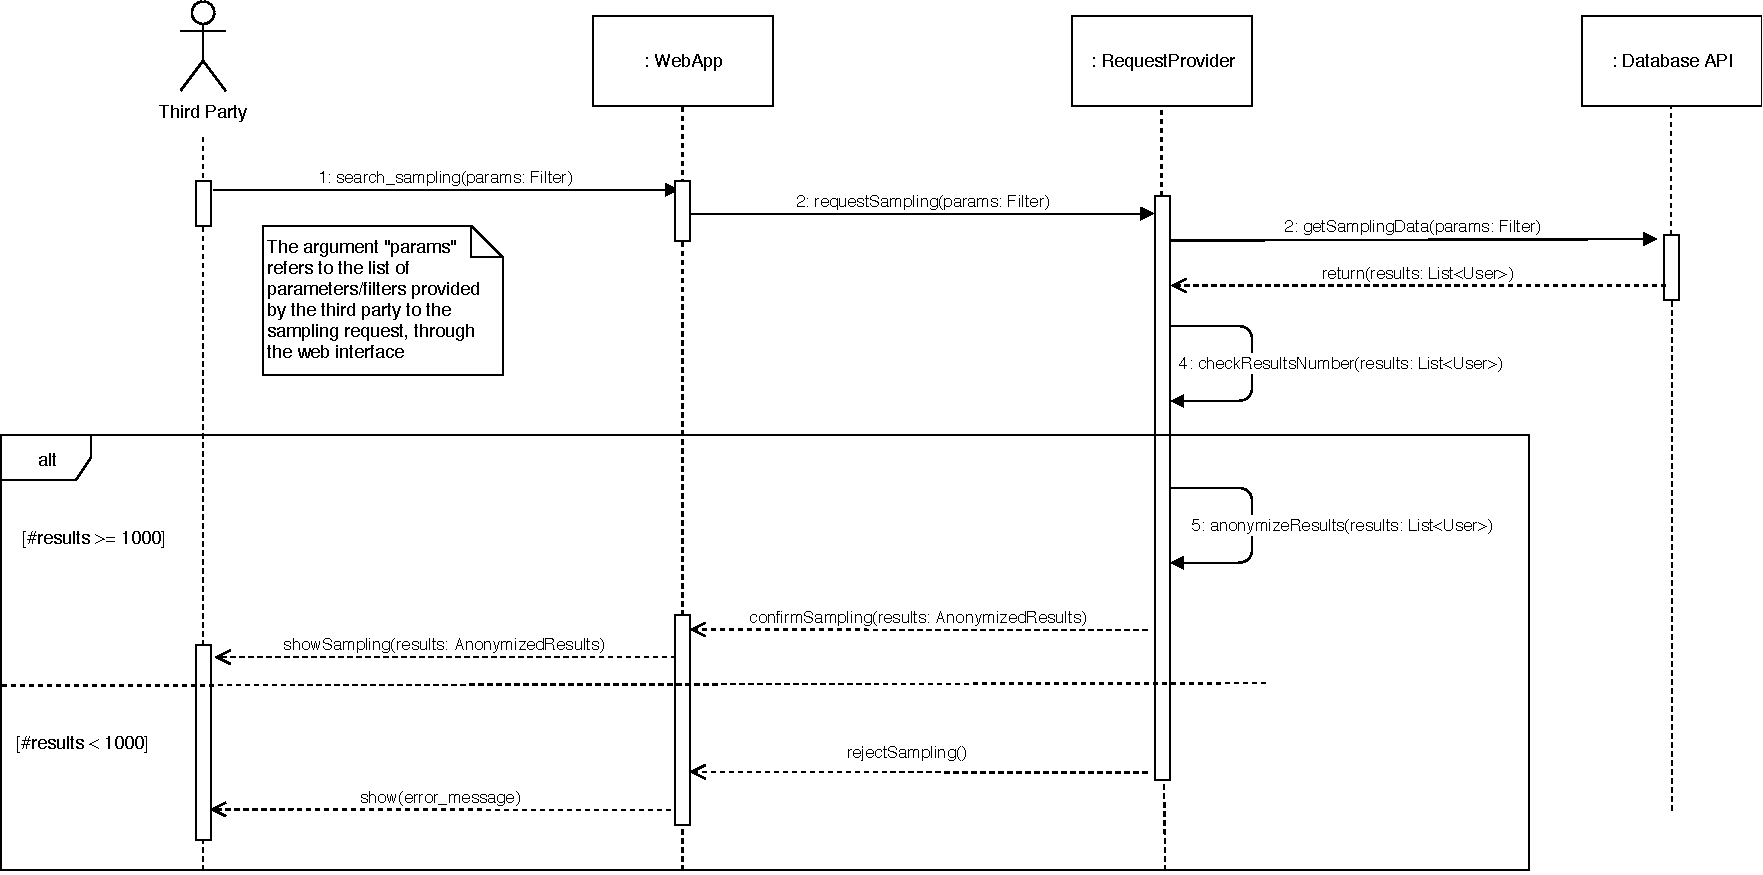
\includegraphics[width=1.0\linewidth]{images/sampling_sequence}
					\label{fig:samplingsequence}
				\end{figure}
			In this sequence diagram the sampling search process is shown. The main component of this process is the RequestProvider. The process begins when a third party, through the Web App, can click on the sampling button and a sampling request is then forwarded to the RequestProvided which in turn gets sampled data from the database and returns the results to the RequestProvided. When sampled data is returned, the RequestProvider checks if the number of sampled people is greater or equal that 1000. If this is the case, the results are notified to the third party, otherwise an error message is shown.
				
		
		\newpage
		\subsection{Architectural Styles and Design Patterns}
			\subsubsection{Design Patterns}
				In order to better formalize our architecture and make it as flexible as possible and speed up the devolpment process of our system we used different design patterns:
				\begin{itemize}
					\item \textbf{Model View Controller}\\ 
					The majority of Mobile and Web applications rely on this pattern. In fact, these applications retrieve data from a data collector (generally a Database) and update the User Interface, according to the input provided and the validity of the requested operation is checked by the Controller.\\
					Thus, the main key of this pattern is to create a separation between the User Interface (View), the data (Model) and the response and validity checking of the User's input (Controller).
						\begin{figure}[H]
							\centering
							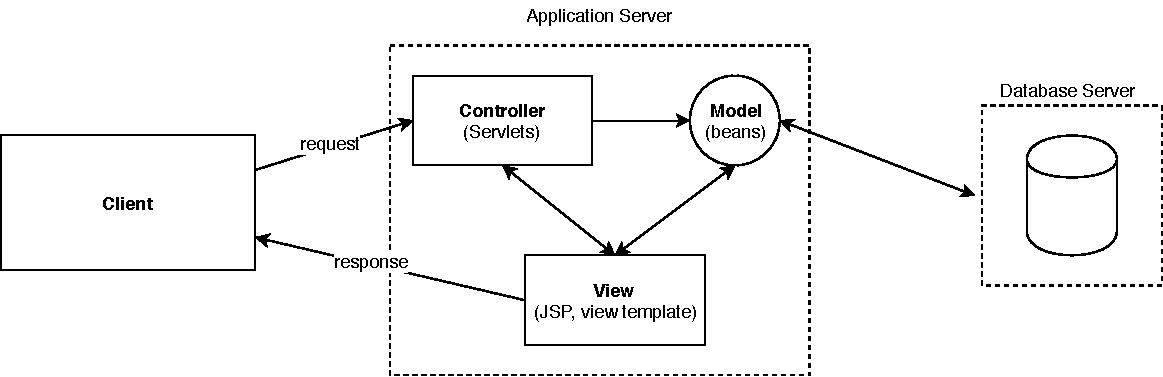
\includegraphics[width=0.7\linewidth]{images/mvc}
							\caption{Distributed MVC in the context of Java EE.}
							\label{fig:mvc}
						\end{figure}
					\item \textbf{Observer and Observable}\\
					In this pattern, there are many observers (objects) which are observing a particular subject (observable object). Observers are basically interested and want to be notified when there is a change made inside that subject. So, they register themselves to that subject. When they lose interest in the subject they simply unregister from the subject. In our system, the intent of this pattern is to let the User execute some query through the UI and after searching the Database, the result is reflected back in the UI. In most of the cases we segregate the UI with the Database. If a change occurs in the database, the UI should be notified so that it can update its display according to the change. When a change is occurring an event is notified and the changes are applied and updated for the User.\\ 
					When referring to a distributed system, this pattern is called Pub-Sub (\textbf{Publish-Subscribe}). 
					\item \textbf{Fa�ade Pattern}\\
					This design pattern supports loose coupling. In fact we emphasize the abstraction and hide complex details by exposing a single interface instead of multiple ones. According to our system we expose to the client \texttt{ThirdPartyWebServices} and \texttt{UserMobileServices} that are in turn extended respectively by all the interfaces provided by the subsystems Third Party Web Services, User Mobile Services and User Smartwatch Services (see section 3, Component View).
					\item \textbf{Proxy Pattern}\\
					It provides a surrogate for another object to control access to it. In our system architecture it can be useful to interface the Application Server with the Database Server. For example, whenever a user or a third party requests some data that is unchanged, the proxy can answer the query without involving access to the database, providing a better response time. In our case, this is useful to improve service response time, very important in critical services that involve users' health.
				\end{itemize}
			\newpage
			\subsubsection{RAPS Architecture}
			As mentioned briefly in the RASD (sections 3.9.2, 3.9.5), our system has to rely on a RAPS (\texttt{Reliable Array of Partitioned Service}) architecture, in order to prevent unavailability of some functionalities in case of breakdowns. This architecture consists in a partitioned and redundant structure: servers are cloned to achieve this objective.
			More precisly, multiple services are divided on different machines and each machine can access in turn to a copy of the stored data. Such architecture guarantees better availability and scalability and provides a high rate of maintainability: in case of breakdowns, it is sufficient to work on the damaged machine, without interfering with the other machines' tasks, while the specific service can still be perfomed. 
			In addition, if the system is willing to expand some services, it is sufficient invest on the specific partition associated to that service.
			\begin{figure}[H]
				\centering
				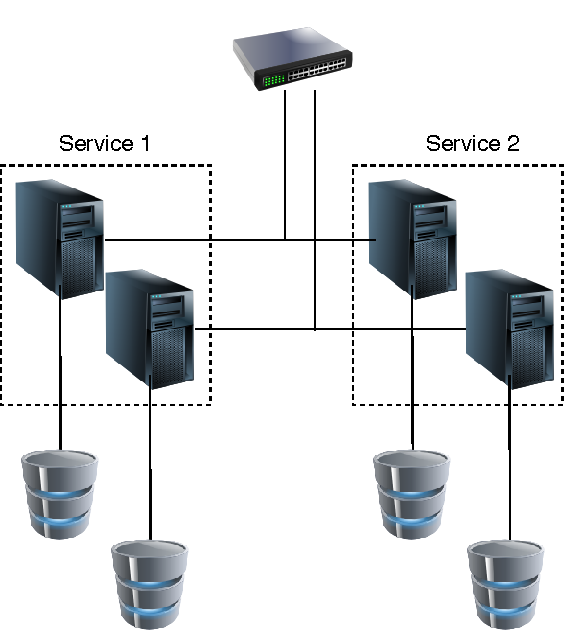
\includegraphics[width=0.6\linewidth]{images/raps}
				\caption{RAPS Architecture}
				\label{fig:raps}
			\end{figure}
			\newpage
			\subsubsection{Transactions Commit Protocol}
				Since our system is likely to use more than one single node for the Database Server, that communicate with one or more Application Server nodes, a non-blocking distributed protocol for transaction should be selected. An example is the Three-Phase Commit Protocol (3PC): the protagonists are a Coordinator (Transaction Manager, TM) and several Participants/Cohorts (Resource Manager, RM). Thanks to a third phase (with respect to the simple Two-Phase Commit Protocol, 2PC), each participant can become a coordinator in case of failure of the TM itself. This allows 3PC to been non-blocking, while 2PC would block in case of failure of both the coordinator or a participant. This protocol also ensures that whenever a transaction is holding some resources, it will release the lock after a timeout, trying to avoid possible deadlocks (see section 7.1 Reference Documents for more details).
		
		\subsection{Other Design Decisions}
			For what concerns the Mobile App, we decided not provide a cross-platform web based application, using some framework/library such as React.js, even though it can save time since the code can be reused for different platforms. \\
			Due to the fact that our application must interface with some wearable devices, we prefer providing native applications, both for Android and iOS.
			Doing so the developed applications can guarantee a better performance during their execution and a better user experience: a user who is used to, for example, the iOS graphical interface, will feel more comfortable using an app with the same type of GUI components.\\
			Furthermore, native applications guarantee their optimal integration with one another and with the entire ecosystem (referring for example to an Apple Watch paired to an iPhone device).
			
		
	\newpage
	\section{User Interface Design}
		As already mentioned in the texttt{Requirements Analysis and Specification Document} (RASD) the idea is to provide a Mobile App for individual users, both for smartphone and for smartwatch, while TrackMe just have a Web Interfaces for third parties. This choice has been driven by the idea that it would be more comfortable for third party companies, since their employees can access the system through their office laptop or desktop PC.
		\\ \\
		For a render of how we thought the user experience should look like, we refer to the specification document in which some mockups have been presented (section 3.1.1, page 13).
	
	\newpage
	\section{Requirements Traceability}
		\subsubsection*{[G1]: Allow visitors to easily register in the system and later to login}
				\begin{itemize}
					\begin{itemize}
						\item Requirements:
							\begin{itemize}
								\item {[R1] - [R5]}
							\end{itemize}
						\item Components: 
							\begin{itemize}
								\item {Profile Manager Module}
								\item {Authentication Manager Module}
							\end{itemize}
					\end{itemize}
				\end{itemize}
		\subsubsection*{[G2]: Allow Users to share personal information/health parameters}
				\begin{itemize}
					\begin{itemize}
						\item Requirements:
							\begin{itemize}
								\item {[R6] - [R8]}
							\end{itemize}
						\item Components: 
							\begin{itemize}
								\item {Profile Manager Module}
								\item {Activity Tracker Module}
							\end{itemize}
					\end{itemize}
				\end{itemize}
		\subsubsection*{[G3]: Allow Third Parties to access information shared by the Users}
				\begin{itemize}
					\item {[G3.1]: Allow Third Parties to access information of specific individuals}
					\begin{itemize}
						\item Requirements:
							\begin{itemize}
								\item {[R9] - [R11]}
							\end{itemize}
						\item Components:
							\begin{itemize}
								\item {Access Requests Module}
								\item {Individual Requests Module}
								\item {Data Access Module}
							\end{itemize}
					\end{itemize}
				\end{itemize}
				\begin{itemize}
					\item {[G3.2]: Allow Third Parties to access anonymized information and parameters of groups of individuals}
					\begin{itemize}
						\item Requirements:
							\begin{itemize}
								\item {[R12] - [R14]}
							\end{itemize}
						\item Components:
							\begin{itemize}
								\item {Sampling Requests Module}
							\end{itemize}
					\end{itemize}
				\end{itemize}
				\begin{itemize}
					\item {[G3.3]: Allow Third Parties to subscribe to new information of a specific individual and to receive it}
					\begin{itemize}
						\item Requirements:
							\begin{itemize}
								\item {[R15] - [R16]}
							\end{itemize}
						\item Components:
							\begin{itemize}
								\item {Subscription Module}
								\item {Data Access Module}
							\end{itemize}
					\end{itemize}
				\end{itemize}
		\subsubsection*{[G4]: Guarantee users an assistance service when necessary}
				\begin{itemize}
					\item {[G4.1]: Guarantee the elderly users to receive an immediate assistance by an ambulance in case of high risk disease}
					\begin{itemize}
						\item Requirements:
							\begin{itemize}
								\item {[R17] - [R19]}
							\end{itemize}
						\item Components:
							\begin{itemize}
								\item {Profile Manager Module}
								\item {Activity Tracker Module}
								\item {Health Monitoring Module}
								\item {SOS Assistance Module}
							\end{itemize}
					\end{itemize}
				\end{itemize}
				\begin{itemize}
					\item {[G4.2]: Allow users to request on-demand ambulance assistance}
					\begin{itemize}
						\item Requirements:
							\begin{itemize}
								\item {[R18] - [R20]}
							\end{itemize}
						\item Components:
							\begin{itemize}
								\item {Activity Tracker Module}
								\item {SOS Assistance Module}
							\end{itemize}
					\end{itemize}
				\end{itemize}
		\subsubsection*{[G5]: Guarantee the preservation of the privacy of the Users}
				\begin{itemize}
 					\begin{itemize}
						\item Requirements: 
							\begin{itemize}
								\item {[R5]}
								\item {[R14]}
								\item {[R21] - [R24]}
							\end{itemize}
						\item Components:
							\begin{itemize}
								\item {Profile Manager Module}
								\item {Authentication Manager Module}
								\item {Access Requests Module}
								\item {Sampling Requests Module}
							\end{itemize}
					\end{itemize}
				\end{itemize}
			
	
	\newpage
	\section{Implementation, Integration and Test Plan}
		\subsection{Implementation Plan}
		The implementation of our system will be done component by component and module by module, according to a bottom-up approach that will facilitate a high deployment coverage in early phases. The order in which our implementation will be carried out, takes in account different factors such as the complexity of the modules and how they are interconnected with one another and we must take in consideration the possibility of discovering flaws and bugs in our designed system that will require to be fixed as soon as possible in order to prevent further additional costs and difficulties in debugging.\\\\
		Hence, we can group the system components as follows:
		\begin{itemize}
			\item \textbf{Model}:
			This component is the first one that must be implemented since all the parts of the Application Server will be using its elements and it allows services to communicate with the DBMS and thus, it is a very important and crucial component for the whole system.\\\\
			The following two components can be identified as the most crucial of the system and their implementation is required to be accomplished as soon as possible since they enclose all the functionalities required both for Users and for Third Parties, and for this reason their fulfillment will require a significative amount of time.
			\item \textbf{User Mobile Services}: This macro-component, along with the \texttt{Third Party Web Services} component is the most complex and most important of the system, due to its functionalities of providing all the services necessary for the User. The functionalities provided are achieved by means of different internal modules, identified as follows: \texttt{ActivityTrackerModule}, \texttt{HealthMonitoringModule}, \texttt{SOSAssistanceModule}, \texttt{AccessRequestsModule} and \texttt{ProfileManagerModule}.
			\item \textbf{Third Party Web Services}: Likewise, this macro-component is very complex and its functionalities provide all the services necessary for Third Parties. The functionalities provided are achieved by means of different internal modules, identified as follows: \texttt{DataAccessModule}, \texttt{SubscriptionModule}, \texttt{IndividualRequestsModule}, \texttt{SamplingRequestsModule} and \texttt{AuthenticationManagerModule}.
			\newpage
			\item \textbf{Client and Router}: These components are used to redirect requests and offer the User a way to communicate with the modules and services which will be carrying out the main functions of the system. 
		
			 
		\end{itemize}
		
		\subsection{Integration and Testing}
		In the following sections we are going to illustrate how external components will be integrated with the ones implemented for the system and what testing strategy will be adopted.
			\subsubsection{Entry Criteria}
				The integration of components and its testing should be carried out as soon as possible, although some conditions must be respected before beginning the verification process. 
				\begin{itemize}
					\item In the very first place, the \texttt{Requirements Analysis and Specification Document} and the \texttt{Desing Document} must be complete and available to all the people involved in the development of the system in order to make them aware about requirments and adopted design choices.
					\item External components and API must be available and serviceable even before the beginning of the implementation process.
					\item The modules which are being integrated in the system are supposed to have at least the operations concerning one another created, if not carried out completely. 
					\item The developed operations should, in the first place, pass unit tests to make sure that the components are working properly, and in case of failure, it will be guaranteed that a misfunctioning is located in the integration process itself and it will be consequently much easier to target the problem and solve it.
				\end{itemize} 
				Furthermore, in order to test the integration of two generic components, the main featues of both of them should have been developed (partially, if not completely) and the related unit tests should have been performed. More clearly, there are minimum percentages of completion of each component with its functionalities that have to be reached in order to perform meaningful integration tests:
				\begin{itemize}
					\item 70\% of the ActivityTrackerModule (must be enough accurate to test if it is really working, so the majority of its functions should be completed).
					\item 70\% of the HealthMonitoringModule (it is one of the most critical parts, it must be almost completed to give a decent accuracy).
					\item 80\% of the SOSAssistanceModule (all features are expected to be implemented completely except for minor ones, such as checking ETA).
					\item 80\% of the AccessRequestsModule (most of the feature should be implemented, since it is crucial to guarantee users' privacy).
					\item 60\% of the ProfileManagerModule (at least the feature of editing the most important information of a User).
					\item 60\% of the DataAccessModule (it deals with users' data, so it is expected to be at least half completed).
					\item 60\% of the SubscriptionModule (at least the subscription feature itself).
					\item 80\% of the IndividualRequestsModule (it is the counterpart of the AccessRequestsModule, so most of its functionalities should be implemented).
					\item 60\% of the SamplingRequestsModule (at least half of the possible search filters should be available).
					\item 60\% of the AuthenticationManagerModule (at least the authentication feature itself, ignoring in the very first place functionalities such as password recovery).
				\end{itemize}
			\subsubsection{Elements to be Integrated}
				The system is composed by the components previously described and will be integrated as follows:
				\begin{itemize}
					\item \texttt{Integration of the components with the DBMS}
					\item \texttt{Integration of the components with external services}
					\item \texttt{Integration of the components of the Application Server}
					\item \texttt{Integration of the Client side with the Application Server}
				\end{itemize}
				\newpage
				\begin{itemize}
					\item \textbf{Integration of the components with the DBMS}\\
					The required integrations are the following:
					\begin{itemize}
						\item \texttt{ActivityTrackerModule, DBMS}
						\item \texttt{SOSAssistanceModule, DBMS}
						\item \texttt{AccessRequestsModule, DBMS}
						\item \texttt{ProfileManagerModule, DBMS}
						\item \texttt{DataAccessModule, DBMS}
						\item \texttt{SubscriptionModule, DBMS}
						\item \texttt{IndividualRequestsModule, DBMS}
						\item \texttt{SamplingRequestsModule, DBMS}
						\item \texttt{AutheticationManagerMoudle, DBMS}
					\end{itemize}
			
					\item \texttt{Integration of the components with external services}\\
					The required integrations are the following:
					\begin{itemize}
						\item \texttt{ActivityTrackerModule, MapsService}
						\item \texttt{ActivityTrackerModule, SensorsService}
						\item \texttt{SOSAssistanceModule, AmbulanceDispatchingSystem}
						\item \texttt{SOSAssistanceModule, NotificationsService}
						\item \texttt{AccessRequestsModule, NotificationsService}
						\item \texttt{ProfileManagerModule, SMSService}
						\item \texttt{SubscriptionModule, NotificationsService}
						\item \texttt{IndividualRequestsModule, NotificationsService}
					\end{itemize}
					\item \texttt{Integration of the components of the Application Server}\\
						The required integrations are the following:
						\begin{itemize}
						\item \texttt{HealthMonitoringModule, ActivityTrackerModule}
						\item \texttt{HealthMonitoringModule, SOSAssistanceModule}
						\item \texttt{SubscriptionModule, DataAccessModule}
						\item \texttt{DataAccessModule, ActivityTrackerModule}
						\item \texttt{IndividualRequestsModule, AccessRequestsModule}
					\end{itemize}
					\item \texttt{Integration of the Client side with the Application Server}\\
					This integration is accomplished to enable the sending of requests between the Server side and the App used by the User.
				\end{itemize}
			
			\newpage
			\subsubsection{Integration Testing Strategy}
				Since the development process follows a bottom-up approach, we decided to use a similar approach for the testing phase: in the very first place we will start by integrating those components that do not depend on other ones in order to work properly, or those who depend on already developed components (such as external API's). After all the single components are tested, we will end up by integrating the subsystems the previous components take part of. This allows us to begin to test a component or a subsystem as soon as it's finished (or near completion), which in turn gives us immediate feedback and allows us to (partially) parallelize the development phase and the testing phase.
				
		\subsection{Application Server Components Integration}
			In this section of the document the order of integration of the components and subsystems of TrackMe system will be described.
			As a notation, an arrow going from component A to component B means that A is necessary for B to function, so it must have already been implemented before performing the integration.
			\begin{figure}[H]
				\centering
				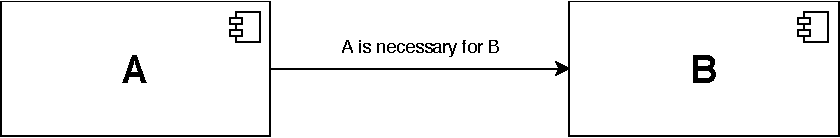
\includegraphics[width=0.7\linewidth]{images/BneedsA}
				\label{fig:bneedsa}
			\end{figure}
			\subsubsection{User side Integration sequence}
				
				\begin{figure}[H]
					\centering
					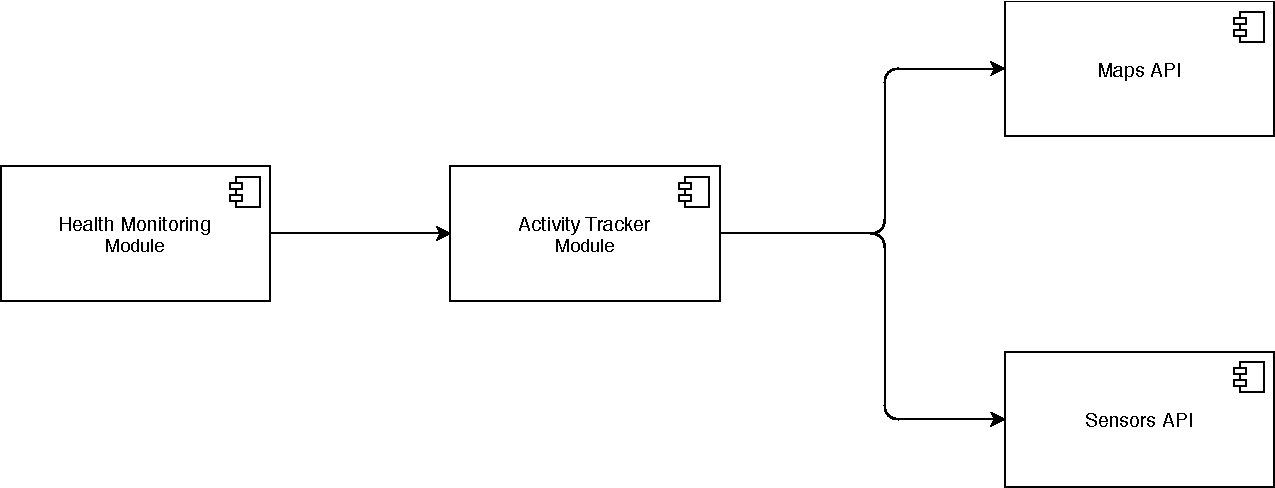
\includegraphics[width=0.7\linewidth]{images/activity_tracker_integration}
					\caption{Activity Tracker}
					\label{fig:activitytrackerintegration}
				\end{figure}
				
				\begin{figure}[H]
					\centering
					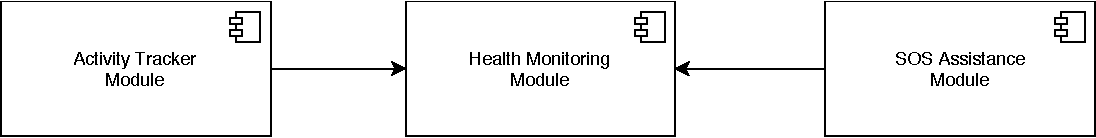
\includegraphics[width=0.7\linewidth]{images/health_monitoring_integration}
					\caption{Health Monitoring}
					\label{fig:healthmonitoringintegration}
				\end{figure}
				
				\begin{figure}[H]
					\centering
					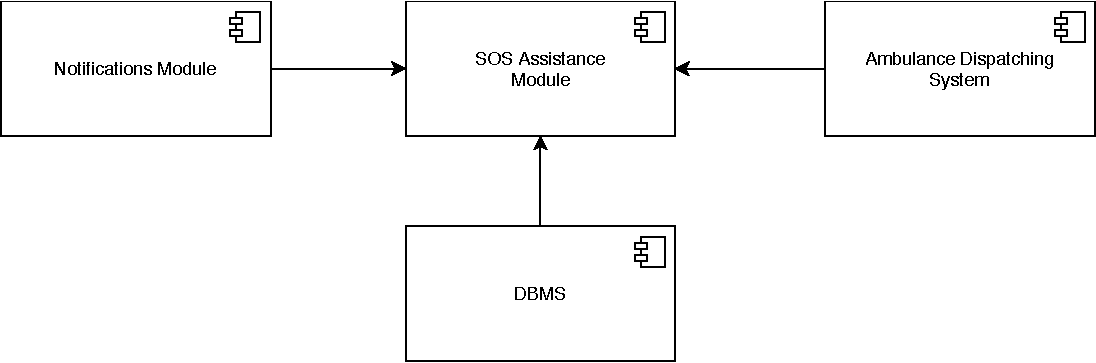
\includegraphics[width=0.7\linewidth]{images/sos_integration}
					\caption{SOS Assistance}
					\label{fig:sosintegration}
				\end{figure}
				
				\begin{figure}[H]
					\centering
					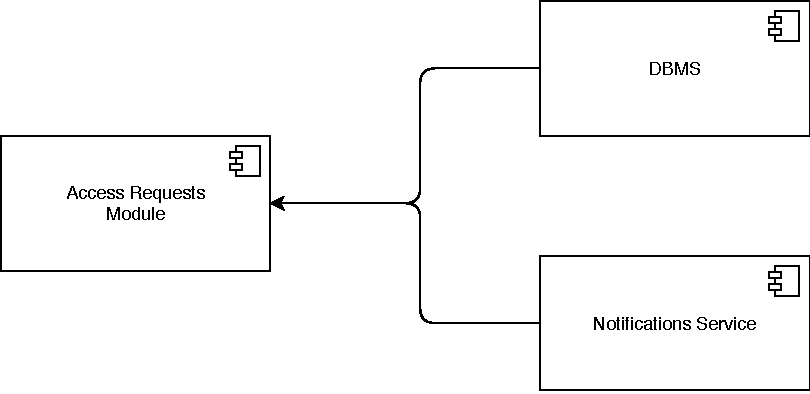
\includegraphics[width=0.7\linewidth]{images/access_request_integration}
					\caption{Access Requests}
					\label{fig:accessrequestintegration}
				\end{figure}
				
				\begin{figure}[H]
					\centering
					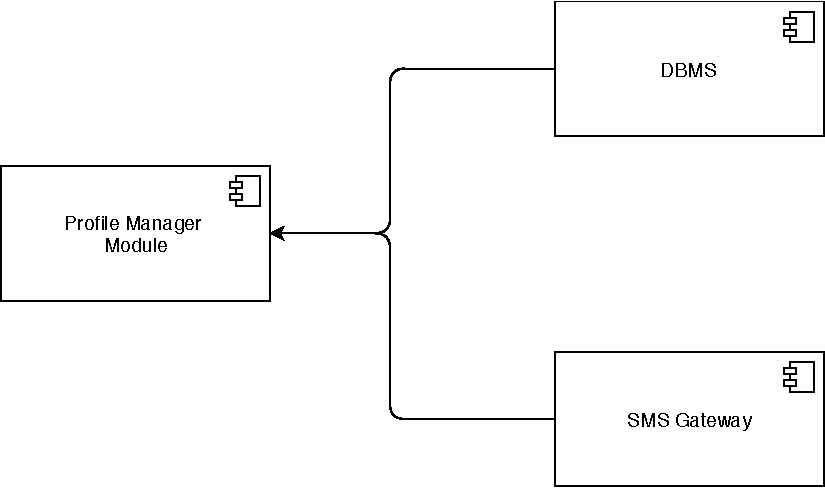
\includegraphics[width=0.5\linewidth]{images/profile_manager_integration}
					\caption{Profile Manager}
					\label{fig:profilemanagerintegration}
				\end{figure}
		
			\subsubsection{Third Party side Integration sequence}
				\begin{figure}[H]
					\centering
					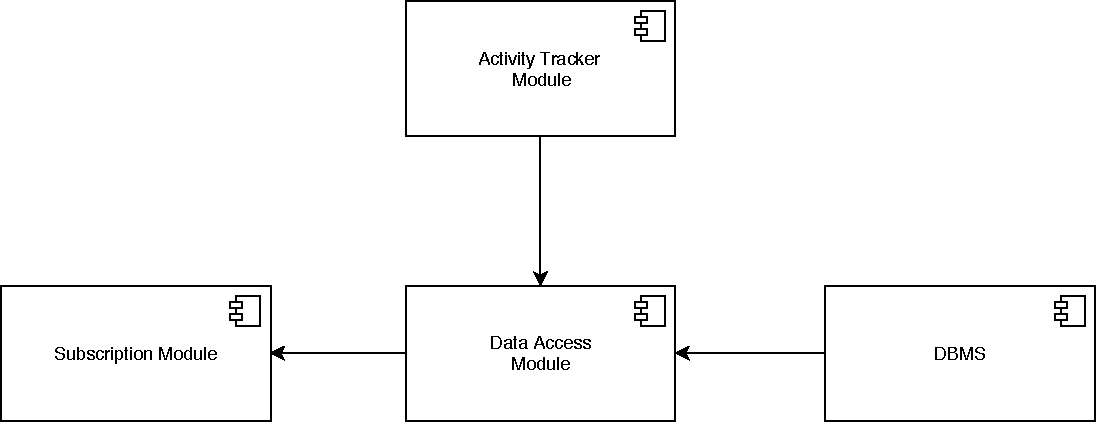
\includegraphics[width=0.7\linewidth]{images/data_access_integration}
					\caption{Data Access}
					\label{fig:dataaccessintegration}
				\end{figure}
			
				\begin{figure}[H]
					\centering
					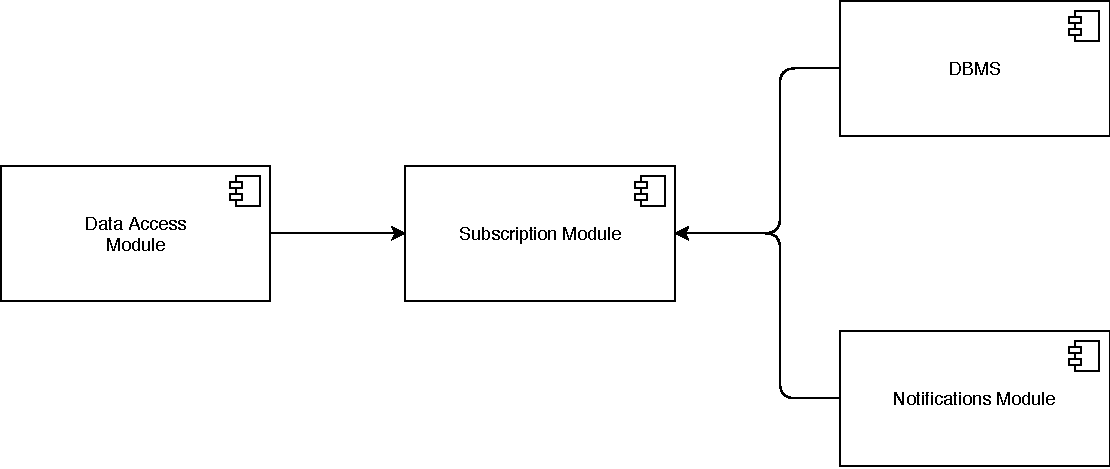
\includegraphics[width=0.7\linewidth]{images/sub_integration}
					\caption{Subscription}
					\label{fig:subintegration}
				\end{figure}
			
				\begin{figure}[H]
					\centering
					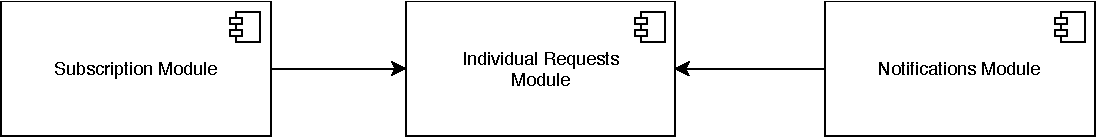
\includegraphics[width=0.7\linewidth]{images/ind_request_integration}
					\caption{Individual Requests}
					\label{fig:indrequestintegration}
				\end{figure}
			
				\begin{figure}[H]
					\centering
					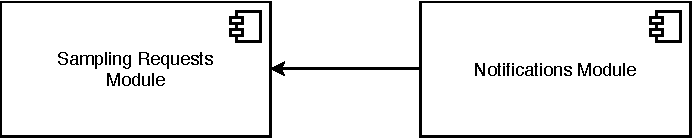
\includegraphics[width=0.7\linewidth]{images/sampling_integration}
					\caption{Sampling Requests}
					\label{fig:samplingintegration}
				\end{figure}
			
				\begin{figure}[H]
					\centering
					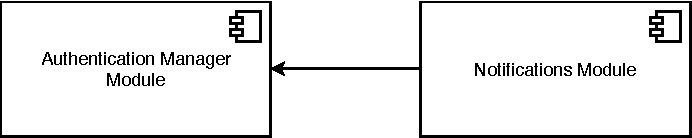
\includegraphics[width=0.7\linewidth]{images/auth_integration}
					\caption{Authentication Manager}
					\label{fig:authintegration}
				\end{figure}
			
	\newpage
	%\section{Appendix}
	\section{Effort Spent}
	\begin{itemize}
		\item Luca Conterio
		\begin{center}
			\begin{tabular}{| c | c | c |}
				\hline
				Day & Subject & Hours \\ \hline
				19/11/2018 & High Level Components & 1.5 \\
				22/11/2018 & Component View & 1.5 \\
				25/11/2018 & Component View & 3 \\
				26/11/2018 & Deployment View & 2.5 \\ 
				27/11/2018 & Deployment View & 2 \\ 
				29/11/2018 & Component Interfaces & 1.5 \\ 
				02/12/2018 & Runtime View & 2 \\ 
				04/12/2018 & Runtime View & 3 \\ 
				06/12/2018 & UML Class Diagram & 2 \\ 
				08/12/2018 & Requirements Traceability & 1 \\ 
				10/12/2018 & Document review & 4 \\ \hline
				Total &									& 24 \\ \hline
			\end{tabular}
		\end{center}

		\item Ibrahim El Shemy
		\begin{center}
			\begin{tabular}{| c | c | c |}
				\hline
				Day & Subject & Hours \\ \hline
				19/11/2018 & Introduction of the document & 1.5 \\ 
				22/11/2018 & Component View & 3 \\ 
				25/11/2018 & Component View & 3 \\ 
				26/11/2018 & Deployment View & 2.5 \\ 
				27/11/2018 & Deployment View and Design Patterns & 2.5 \\ 
				04/12/2018 & Implementation, Integration and Test Plan & 2 \\  
				05/12/2018 & Implementation, Integration and Test Plan & 3 \\ 
				08/12/2018 & Integration Diagrams & 4 \\ 
				10/12/2018 & Document review & 4 \\  \hline
				Total &									& 25.5 \\  \hline
			\end{tabular}
		\end{center}
	\end{itemize}

	\newpage
	\section{References and Used Tools}
		\subsection{Reference Documents}
			\begin{itemize}
				\item Specification Document "Mandatory Project Assignment A.Y. 2018/2019"
				\item "Appunti di Sistemi Informativi per il Settore dell'Informazione" A.Y. 2017/2018
				\item "Java Design Patterns", Vaskaran Sarcar
				\item Software Engineering 2 course slides
				\item Data Bases 2 course slides
				\item "https://developer.jboss.org/wiki/Three-phaseCommitProtocol"
			\end{itemize}
		\subsection{Tools}
			\begin{itemize}
				\item \textbf{Draw.io}: \texttt{https://www.draw.io/}
				\item \textbf{TeXStudio}: \texttt{http://www.textstudio.org/}
				\item \textbf{Github}: \texttt{https://github.com/}
			\end{itemize}
		
\end{document}
